\chapter{Commande proportionnelle intégrale de DarkO}
\todo{Vendre du rêve}
\minitoc
\label{chap:6DOF}

\section{Motivation}
\label{sec:motivation6DOF}
Nous avons observé expérimentalement dans le chapitre \ref{chap:3DOF} qu'un drone \textit{tailsitter} pouvait se stabiliser en stationnaire face à du vent, vers les points d'équilibre décrits dans la section \ref{sec:eq_vent}, grâce à une architecture de commande linaire. Cette dernière est basée sur un retour de sortie, proportionnel intégral, libérant deux degrés de liberté sur l'orientation du drone.


\section{Commande linéaire proportionnelle intégrale}
\label{sec:6dofcmd}
\subsection{Description du schéma de contrôle}
\label{sec:ctl_sche}

Une inspection minutieuse des matrices de commande et d'entrée des perturbations $\boldsymbol{G}_{w}$ et $\boldsymbol{E}_{w}$ du modèle \eqref{eq:lpv_linearisation} (voir la sortie de l'Algorithme~\ref{alg:linea}) suggère une architecture de contrôle efficace pour rejeter une perturbation de vent constante $\boldsymbol{w}$. En effet, les ailerons et les hélices peuvent être utilisés symétriquement pour générer respectivement un moment autour de l'axe $y_{[\text{b}]}$, vérifiant l'équation \eqref{eq:momenty}, et une force le long de l'axe $x_{[\text{b}]}$, vérifiant l'équation \eqref{eq:forcex}, compensant ainsi l'effet de la perturbation. Néanmoins, il reste une force le long de l'axe $z_{[\text{b}]}$ à compenser en vérifiant l'équation \eqref{eq:forcez}. Une action intégrale peut converger asymptotiquement vers la force désirée, même avec une perturbation du vent non mesurée ($\boldsymbol{w}$). Nous pouvons donc stabiliser le drone à l'équilibre en vol stationnaire tel que caractérisé dans le Théorème~\ref{thm:eqs}. Comme nous ne mesurons pas le vent $\boldsymbol{w}$, les valeurs de $\psi$ et $\theta$ dans l'Algorithme~\ref{alg:eq} sont inconnues. Le contrôleur proposé, illustré à la Fig.~\ref{fig:commande_int6DOF}, utilise l'action intégrale pour faire converger ces angles vers leur valeur d'équilibre. Le bouclage utilise les variables d'erreur suivantes : 
\begin{align}
    \boldsymbol{e}_{p}= \boldsymbol{r}_{p} - \boldsymbol{p}, \; \boldsymbol{e}_{v \epsilon \omega} = -  
       \left[ \begin{smallmatrix} \mathbb{I}_{3}  & \mathbb{0}_{3\times 1} & \mathbb{0}_{3\times 2} & \mathbb{0}_{3}\\
       \mathbb{0}_{1\times 3}  & 1 & \mathbb{0}_{1\times 2} & \mathbb{0}_{1 \times 3} \\
           \mathbb{0}_{3}  & \mathbb{0}_{3\times 1} & \mathbb{0}_{3\times 2} &   \mathbb{I}_{3}
           \end{smallmatrix} \right]
    \smallmat{
           \tilde{\boldsymbol{v}} \\
           \tilde{\boldsymbol{\epsilon}} \\
           \tilde{\boldsymbol{\omega}}_{\text{b}} 
    }.
  \label{eq:error_var}
\end{align} 

Ces variables d'erreur doivent converger vers zéro dans le cas d'un vol stationnaire et pour n'importe quelle position de référence constante $\boldsymbol{r}_{p} \in \mathbb{R}^{3}$. Notons que $\boldsymbol{r}_{p}$ est l'entrée de référence du schéma de contrôle.

Les variables d'erreur dans \eqref{eq:error_var} peuvent être représentées comme dans le schéma  de la Fig.~\ref{fig:commande_int6DOF}, c'est-à-dire, en définissant la sortie $\boldsymbol{y}\in \real^{10}$ de la dynamique du système linéarisé \eqref{eq:lpv_linearisation}, ayant le vecteur d'état incrémental $\boldsymbol{\tilde{x}} \in \real^{10 \times 1}$ défini ci-dessous : 
\begin{align}
    \label{eq:output_lin}
    \boldsymbol{y} = \boldsymbol{C} \boldsymbol{\tilde{x}} + \smallmat{\boldsymbol{p}_{\mathrm{eq}} \\ \mathbb{0}_{7 \times 1}}, \quad
 \boldsymbol{C} := \smallmat{\mathbb{I}_{6} & \mathbb{0}_{6\times 1} & \mathbb{0}_{6\times 2} &\mathbb{0}_{6\times 3}\\
    \mathbb{0}_{1\times 6} & 1 & \mathbb{0}_{1\times 2} &\mathbb{0}_{1\times 3}\\
    \mathbb{0}_{3\times 6} & \mathbb{0}_{3\times 1} & \mathbb{0}_{3\times 2} &  \mathbb{I}_{3}
},
\end{align}
où la matrice de sortie $\boldsymbol{C} \in \real^{10\times12}$ enlève la composante $\tilde{\epsilon}_{2}$ et $\tilde{\epsilon}_{3}$ du vecteur d'état $\tilde{\boldsymbol{x}}$. 

\begin{figure}[t!]
    \centering
    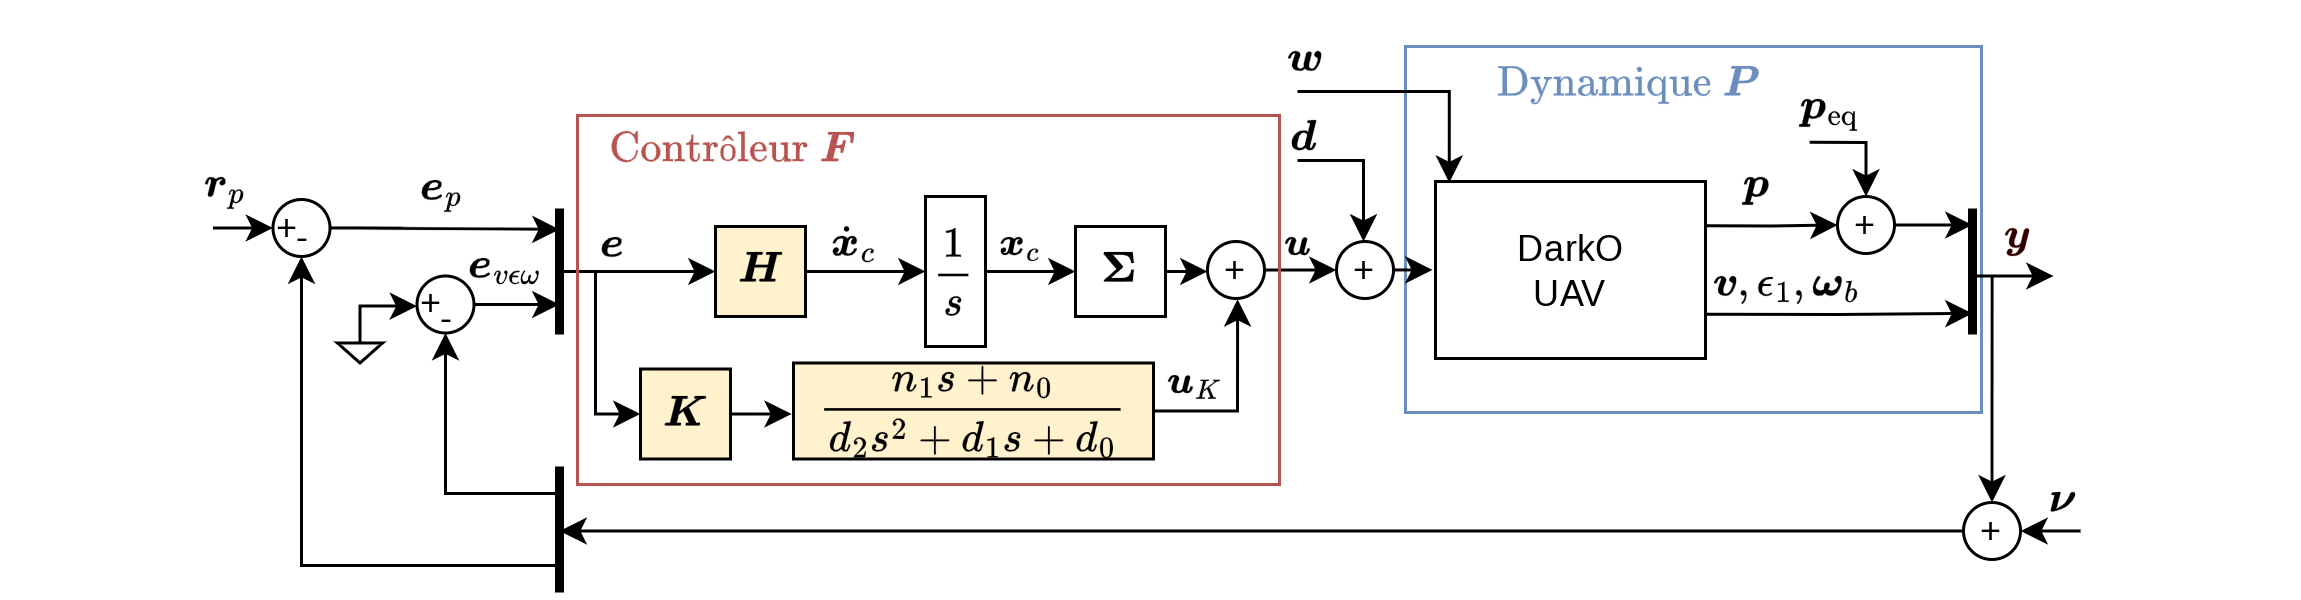
\includegraphics[width=0.8\columnwidth]{figures/commande_integrale.png}
    \caption{Schéma de commande intégrale avec la perturbation de vent $\boldsymbol{w}$, la perturbation du système à l'entrée $\boldsymbol{d}$ et à la sortie $\nu$.}
    \label{fig:commande_int6DOF}
\end{figure}

Comme le montre la Figure~\ref{fig:commande_int6DOF}, les équations de la dynamique du contrôleur sont basées sur l'erreur $\boldsymbol{e}$ suivante :

\begin{subequations}
    \label{eq:contoller}
    \begin{align}
        \boldsymbol{e} = \smallmat{
        \boldsymbol{e}_{p}^\top & \boldsymbol{e}_{v\epsilon\omega}^\top}^\top, \quad \dot{\boldsymbol{x}}_{c} = \boldsymbol{H} \boldsymbol{e}, \quad    \boldsymbol{u} = \boldsymbol{\Sigma} \boldsymbol{x}_{c} + \boldsymbol{u}_{K},
        \\
        \boldsymbol{\Sigma} := \begin{bmatrix} \! 1 \!&\! 1\! & \!0\! &\! 0\!\\ \!0\! & \!0\! & \!1 \!& \!1\!\end{bmatrix}^\top, \quad
        \boldsymbol{u}_{K} = \frac{n_1 s+n_0}{d_2 s^{2}+d_1 s + d_0}\boldsymbol{K} \boldsymbol{e} ,
    \end{align}
\end{subequations}
où $\boldsymbol{x}_{c} \in \mathbb{R}^{2}$ est l'état intégral, $\boldsymbol{\Sigma}$ est une matrice d'allocation des entrées qui permet d'affecter la première composante de l'état de l'intégrateur à l'action des hélices et la deuxième composante à l'action des élevons. Les scalaires $n_1$, $n_0$,  $d_2$,  $d_1$,  $d_0$ sont respectivement les coefficients du numérateur et du dénominateur d'un filtre utilisé pour éviter une transmission directe entrée-sortie qui amplifierait le bruit de mesure à haute fréquence. Ce filtre induit un contrôleur strictement propre, pour une robustesse accrue aux incertitudes additives. 

Nous définissons le contrôleur $\boldsymbol{F}$ ayant pour dimensions 4\texttimes10 avec la matrice de transfert $\boldsymbol{F}(s) = T_{\boldsymbol{e} \rightarrow \boldsymbol{u}}(s)$ telle que décrite dans \eqref{eq:contoller} et l'interconnexion détaillée dans la Figure~\ref{fig:commande_int6DOF}. Le système $\boldsymbol{P}$ de dimensions 10\texttimes4 représente la dynamique linéarisée de DarkO. La sortie du système $\boldsymbol{y} \in \real^{10\times1}$ est utilisée comme entrée du contrôleur $\boldsymbol{F}$.

Compte tenu des symétries des actionneurs du drone, nous avons contraint la structure de la matrice $\boldsymbol{K}$ dans \eqref{eq:contoller}, associée à l'action proportionnelle du contrôleur, afin d'utiliser les actionneurs selon leur action physique. Ainsi, $\boldsymbol{K}$ prend la forme : 
\begin{align}
\label{eq:k_struct}
    \!\!\!\boldsymbol{K}_{\text{struct}} \!=\!  \smallmat{
             k_{1}& \shortminus k_{2}& k_{3}&  k_{4}& \shortminus k_{5}&  k_{6}& \shortminus k_{7}&  k_{8}&  k_{9}& \shortminus k_{10}\\
             k_{1}&  k_{2}& k_{3}&  k_{4}&  k_{5}&  k_{6}&   k_{7}& \shortminus k_{8}& \shortminus k_{9}&  k_{10}\\
            \shortminus k_{11}& \shortminus k_{12}& k_{13}& \shortminus k_{14}& \shortminus k_{15}& \shortminus k_{16}&   k_{17}& \shortminus k_{18}&  k_{19}& \shortminus k_{20}\\
            \shortminus k_{11}&  k_{12}& k_{13}& \shortminus k_{14}&  k_{15}&  k_{16}&   \shortminus k_{17}&  k_{18}&  k_{19}&  k_{20} 
         }.
\end{align}

La structure précédente s'explique par le comportement physique du drone. Une erreur de position sur l'axe $z_{[\text{i}]}$ du repère inertiel NED (voir Fig.~\ref{fig:darko2}) entraîne une utilisation symétrique des deux hélices, ce qui génère une force le long de l'axe $x_{[\text{b}]}$ du drone. L'utilisation symétrique des deux moteurs se traduit par le même signe dans les coefficients $k_{3}$ et $k_{6}$ des colonnes 3 et 6 de $\boldsymbol{K}$, qui correspondent respectivement aux erreurs de position et de vitesse sur l'axe $z_{[\text{i}]}$. De même, une erreur de position ou de vitesse le long de l'axe latéral du drone $y_{[\text{b}]}$ sera compensée par une utilisation antisymétrique des moteurs, comme le montrent les coefficients $k_{2}$ et $k_{5}$ et leur signe opposé dans les colonnes 2 et 5 de $\boldsymbol{K}$. Une erreur de vitesse angulaire autour de l'axe $x_{[\text{b}]}$ doit être compensée par une utilisation antisymétrique des élevons, comme le montre le coefficient $k_{18}$ de signe opposé dans la colonne 8 de $\boldsymbol{K}$. Des arguments parallèles expliquent les coefficients restants de la matrice $\boldsymbol{K}$ dans \eqref{eq:k_struct}. Toutes ces explications ne sont valables que dans un voisinage de l'équilibre, où le drone se trouve être à la verticale. On comprend aisément que dans d'autres configurations, ces contraintes d'actionnement ne sont plus valides. Un avantage de la structure de \eqref{eq:k_struct} est la réduction du nombre de variables à optimiser, de 40 à 20 gains scalaires, cela se traduisant par une diminution du temps nécessaire à l'optimisation.

La boucle fermée illustrée à la Figure~\ref{fig:commande_int6DOF} est un retour de sortie à dix éléments, comprenant les trois positions, les trois vitesses linéaires, l'un des trois angles d'attitude ($\epsilon_{1}$) et les trois vitesses angulaires. Cette structure peut être considérée comme un bouclage proportionnel-intégral MIMO. Les paramètres à régler dans le contrôleur $\boldsymbol{F}$ \eqref{eq:contoller} sont le gain proportionnel $\boldsymbol{K} \in \real^{4\times10}$ dans \eqref{eq:k_struct}, le gain intégral $\boldsymbol{H} \in \real^{2\times10}$ et les paramètres du filtre $n_1$, $n_0$, $d_2$, $d_1$, $d_0$, comme repérés en jaune sur la Fig.~\ref{fig:commande_int6DOF}. Une méthode de réglage appropriée doit garantir une réjection adéquate des perturbations et une robustesse satisfaisante aux dynamiques non modélisées. Ces deux objectifs conduisent à un compromis car le rejet des perturbations nécessite un réglage agressif tandis que les propriétés de robustesse sont assurées par une stratégie d'atténuation des hautes fréquences.

Nous examinons ensuite deux méthodes de réglage basées sur l'optimisation. La première est issue des idées proposées dans \ref{sec:3dofcmd}, méthode qui ne nécessitait pas la dynamique linéarisée des Théorèmes~\ref{thm:eqs} et~\ref{th:lin}, et est résumée dans la section~\ref{sec:zerowind}. Il s'agit d'une synthèse multiobjectif avec des contraintes $H_{\infty}$, basée sur le modèle de vent nul, discutée dans la section~\ref{sec:eq_nowind} et~\ref{sec:nowind_lin} et détaillée dans \ref{sec:3dofcmd}. Nous montrerons que cette première méthode ne permet pas de stabiliser le drone dans certaines plages de vent, en raison de la méconnaissance de la dynamique caractérisée par les Théorèmes~\ref{thm:eqs} et~\ref{th:lin}. La deuxième méthode de réglage, présentée à la section \ref{sec:h_inf6DOF_multi}, est une synthèse itérative multiobjectif avec des contraintes $H_{\infty}$, basée sur un ensemble de modèles associés à différentes conditions de vent, lesquels sont obtenus des Théorèmes~\ref{thm:eqs} et~\ref{th:lin}, par le biais des Algorithmes~\ref{alg:eq} et~\ref{alg:linea}.


Dans notre validation numérique, présentée dans les sections~\ref{sec:zerowind} et~\ref{sec:h_inf6DOF_multi} (voir en particulier les Fig.~\ref{fig:SimSytuneStruct_zero} et Fig.~\ref{fig:SimSytuneStruct_lpv}), un bruit de mesure est ajouté à la sortie pour produire des résultats numériques semblables aux expérimentaux. Les écarts types des niveaux de bruit adoptés sont indiqués dans la Table~\ref{tab:noise}.
\begin{table}[ht!]
    \centering
    \begin{tabular}{|c|c|c|} 
        \hline
        Grandeurs & Valeurs & Unités\\
        \hline
        $\boldsymbol{p}$ & \SI{2.5e-4}{} & \SI{}{\meter}  \\ 
        \hline
        $\tilde{\boldsymbol{v}}$  & \SI{1.2e-3}{} &  \SI{}{\meter\per\second}  \\ 
        \hline
        $\tilde{\boldsymbol{\epsilon}}$ & \SI{4.7e-4}{} &  \\
        \hline
        $\tilde{\boldsymbol{\omega}}_{\text{b}}$ & \SI{2.7e-3}{} &\SI{}{\radian\per\second}\\
        \hline
    \end{tabular}
    \caption{ Écart-type du bruit pour la modélisation des capteurs en simulation.}
    \label{tab:noise}
\end{table}

En plus de présenter les résultats de la simulation du bouclage linéaire de la Fig. ~\ref{fig:commande_int6DOF} avec le modèle linéarisé \eqref{eq:lpv_linearisation}, dans les sections~\ref{sec:zerowind} et~\ref{sec:h_inf6DOF_multi}, nous simulons également la boucle fermée en remplaçant le modèle linéarisé $\boldsymbol{P}$ par le modèle non linéaire \eqref{eq:dyna_orig}, comprenant la dynamique réelle du drone.

Lorsque l'on remplace le modèle linéarisé par la dynamique non linéaire \eqref{eq:dyna_orig}, dont l'état est $\boldsymbol{x} = (\boldsymbol{p}, \boldsymbol{v}, \boldsymbol{q},\boldsymbol{\omega}_{\text{b}}) \in \real^{13} $, nous remplaçons la sortie linéaire $\boldsymbol{y}$ avec la version non linéaire suivante :
\begin{align}
\label{eq:output}
    \boldsymbol{y}_{\text{NL}} \!=\! \smallmat{\boldsymbol{p}\\
     \boldsymbol{v}\\
     \epsilon_{1}\\
     \boldsymbol{\omega}_{\text{b}}} \!=\! \left[ \begin{smallmatrix} \mathbb{I}_{6} & \mathbb{0}_{6\times 1} & \mathbb{0}_{6\times 1} & \mathbb{0}_{6\times 2} & \mathbb{0}_{3}\\
     \mathbb{0}_{1\times 3} & 0 & 1 & \mathbb{0}_{1\times 2} & \mathbb{0}_{1 \times 3} \\
         \mathbb{0}_{3} & \mathbb{0}_{3\times 1} & \mathbb{0}_{3\times 1} & \mathbb{0}_{3\times 2} &   \mathbb{I}_{3}
         \end{smallmatrix} \right]
         \smallmat{\boldsymbol{R}^\top_{\psi}\boldsymbol{p} \\ \boldsymbol{R}^\top_{\psi}\boldsymbol{v} \\
\boldsymbol{q}_{\mathrm{eq}\psi}^{-1} \otimes \boldsymbol{q} \\
         \boldsymbol{\omega}_{\text{b}}  }.
\end{align}


Dans les sections suivantes, nous notons la marge de module d'une matrice de transfert $s \mapsto T_{v \rightarrow z}$ as $\Delta_m(T_{v \rightarrow z}) = \min\limits_{\omega\in R} \sigma_{\min}(T_{v \rightarrow z}(j\omega))$.



\subsection{Contrôleur optimisé sous contraintes $H_{\infty}$, cas sans vent}
\label{sec:zerowind}

Pour régler le contrôleur dans le cas sans vent, nous utilisons le modèle linéaire du système décrit dans la section~\ref{sec:nowind_lin}, $\boldsymbol{P}(s) = T_{\boldsymbol{u} \rightarrow \boldsymbol{y}}(s)$, obtenu à partir des équations \eqref{eq:linearized} et \eqref{eq:output_lin} tel que :

\begin{align*}
    \boldsymbol{P}(s) = \boldsymbol{C} (s \mathbb{I}_{12} - \boldsymbol{A}_{0})^{-1} \boldsymbol{G}_{0}.
\end{align*} 

En lien avec la Figure~\ref{fig:commande_int6DOF}, nous introduisons des matrices de transfert qui correspondent aux objectifs de robustesse : la fonction de sensibilité en sortie définie par $T_{\nu \rightarrow e}=(\mathbb{I}_{10}+\boldsymbol{P}\boldsymbol{F})^{-1}$ de dimensions 10\texttimes10, telle que $\lVert T_{\nu \rightarrow e} \rVert _{\infty}=\Delta_m(T_{\nu \rightarrow e})^{-1} $ et la fonction de sensibilité en entrée $T_{d \rightarrow u}=(\mathbb{I}_{4}+\boldsymbol{F}\boldsymbol{P})^{-1}$ de dimensions 4\texttimes4, définie par $\lVert T_{d \rightarrow u} \rVert _{\infty}=\Delta_m(T_{d \rightarrow u})^{-1}$.
Par conséquent, la minimisation de la norme $H_{\infty}$ de $T_{\nu \rightarrow e}$ ou de $T_{d \rightarrow u}$ correspond à l'augmentation des marges de module en entrée et en sortie. Étant donné que le système $\boldsymbol{P}$ est MIMO, nous accordons de l'importance aux fonctions de sensibilité en entrée et en sortie qui ne coïncident pas, car $\boldsymbol{P}$ et $\boldsymbol{F}$ ne commutent pas.

Nous définissons aussi la matrice de transfert $T_{\nu \rightarrow u}$ de dimensions 4\texttimes10 liée à l'impact du bruit de mesure $\nu$ sur la commande $\boldsymbol{u}$, e $T_{d \rightarrow y}$ de dimensions 10\texttimes4 représentant l'impact de la perturbation en entrée $\boldsymbol{d}$ sur la sortie du système $\boldsymbol{y}$. 

Nous résolvons le même problème que dans notre travail précédent \ref{eq:pb_optim} en utilisant le logiciel {\tt Systune} \cite{1576856}, mais nous utilisons le diagramme de contrôle présenté dans la section~\ref{sec:ctl_sche} qui comprend un filtre sur l'action proportionnelle et un nombre différent de sorties. Nous incluons également dans le système $\boldsymbol{P}$ la dynamique des actionneurs linéaires discutée dans la section~\ref{sec:saturation}.
\begin{figure}[ht!]
    \centering
    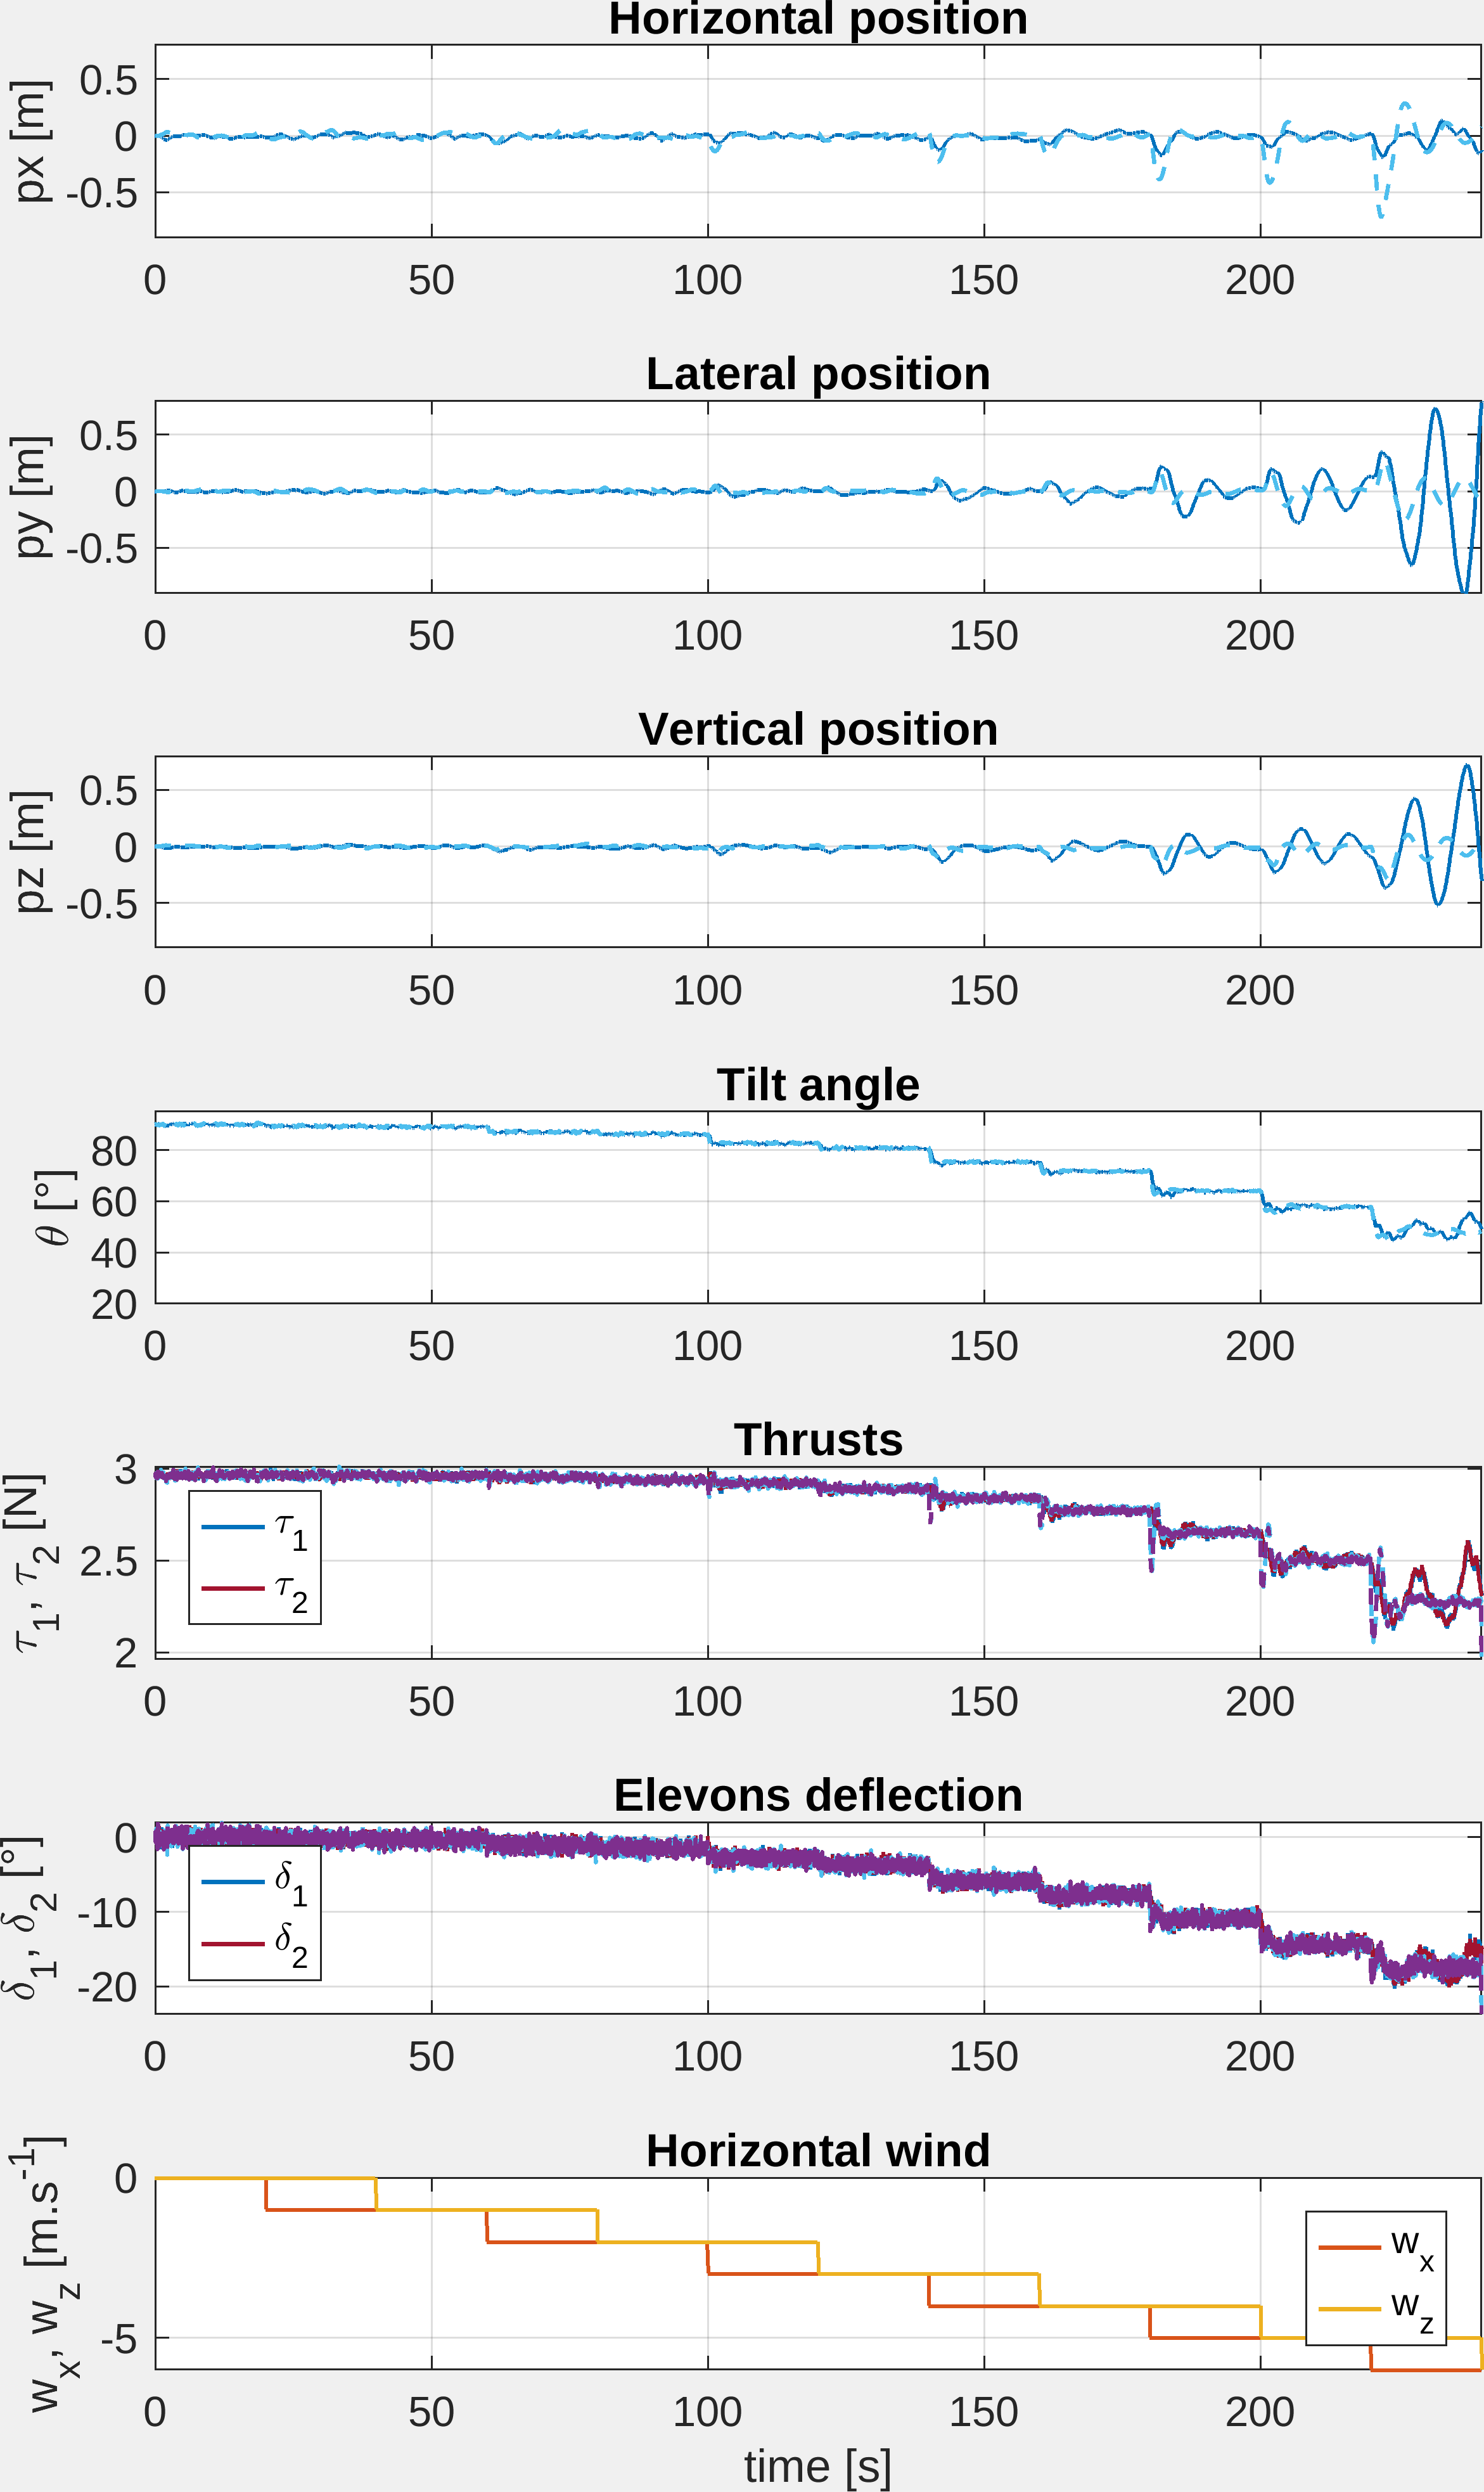
\includegraphics[trim=0cm 0cm 0cm 0cm,clip,width=0.6\columnwidth]{figures/sim_systune_zero_wind.png}
    \caption{Simulation du modèle non linéaire \eqref{eq:dyna_orig} (ligne continue) et du modèle linéarisé \eqref{eq:lpv_linearisation} (ligne en pointillé) avec des incréments de vent constants croissants et le contrôleur basé sur l'optimisation sans vent de la section~\ref{sec:zerowind}.}
    \label{fig:SimSytuneStruct_zero}
\end{figure}

Une augmentation successive de l'intensité horizontale et verticale du vent (allant de 0 à \SI{-6}{\meter\per\second}) est appliquée, comme le montre le tracé inférieur de la Fig.~\ref{fig:SimSytuneStruct_zero}. Les couples de vent sélectionnés $(w_{x}, w_{z})$ sont représentés par des points rouges sur les surfaces de la figure~\ref{fig:saturation}, où l'on peut voir que l'équilibre $(\boldsymbol{u}_{\text{eq}}, \boldsymbol{x}_{\text{eq}})$ est atteint sans que les actionneurs ne soient saturés. Nous ne nous intéressons qu'à la partie négative de la vitesse verticale du vent car elle est la plus limitante. En effet, le drone est soulevé par le vent vertical ascendant (dont le signe est négatif dans le cadre de la NED), nécessitant ainsi moins de traction sur les hélices pour compenser la gravité. Les moteurs génèrent moins de flux d'air sur les élevons, ce qui réduit leur efficacité, conduit à la saturation et déstabilise le drone.
L'objectif du système de contrôle est de maintenir le drone en position de vol stationnaire (définie comme $\boldsymbol{r}_{p} = [0,0,0]^\top$), malgré l'augmentation du vent horizontal et vertical $w_{x}$ et $w_{z}$. 


La Figure~\ref{fig:SimSytuneStruct_zero} présente à la fois des simulations linéaires avec la dynamique linéarisée \eqref{eq:lpv_linearisation} (en pointillé) et des simulations non linéaires avec le modèle non-linéaire \eqref{eq:dyna_orig} (en traits pleins). Les simulations linéaires et non linéaires montrent systématiquement que le contrôleur fonctionne bien à faible vitesse de vent (effectivement, le réglage est effectué sur la base du modèle de vent nul). Cependant, lorsque la vitesse du vent $w_{x}$ et $w_{z}$ dépasse \SI{-5}{\meter\per\second}, la position de vol stationnaire devient instable et le drone oscille et diverge. Les angles d'inclinaison $\theta$ sont utilisés pour représenter l'attitude afin de donner un meilleur aperçu du comportement du véhicule, mais la simulation de la dynamique non linéaire \eqref{eq:dyna_orig} est effectuée avec un quaternion unitaire. L'instabilité observée dans les résultats de la simulation de la figure~\ref{fig:SimSytuneStruct_zero} confirme les instabilités expérimentales rapportées dans la section \ref{sec:exp3DOF}, où nous avons utilisé cette même méthode de réglage. Est également confirmée l'importance des Théorèmes~\ref{thm:eqs} et~\ref{th:lin} dans la Section~\ref{sec:model}, pour un réglage approprié des gains du contrôleur, comme cela est effectué dans la section suivante.


\subsection{Contrôleur optimisé sous contrainte $H_{\infty}$, cas multimodèle}
\label{sec:h_inf6DOF_multi}

Les résultats de simulation obtenus avec la méthode de réglage sans vent (voir la Figure~\ref{fig:SimSytuneStruct_zero}), ainsi que les instabilités expérimentales observées dans la section \ref{sec:exp3DOF} confirment la nécessité d'une procédure de réglage du gain du contrôleur exploitant les linéarisations paramétrées en fonction du vent des Théorèmes~\ref{thm:eqs} et~\ref{th:lin}. En nous concentrant à nouveau sur le schéma de contrôle de la Figure~\ref{fig:commande_int6DOF}, nous considérons maintenant explicitement l'effet du vent (linéarisé) sur le système \eqref{eq:lpv_linearisation} avec la sortie \eqref{eq:output_lin} et avec les sélections de l'algorithme~\ref{alg:linea} comme définies ci-dessous :
\begin{align*}
\label{eq:Pw_synthesis}
\numberthis
    \boldsymbol{P}_w(s) &= \begin{bmatrix}
        \boldsymbol{P}_{u}(s;w) &  \boldsymbol{P}_{w}(s;w)
    \end{bmatrix}\\&:= \boldsymbol{C} (s \mathbb{I}_{12} - \boldsymbol{A}_{w})^{-1} \begin{bmatrix}\boldsymbol{G}_{w} &   \boldsymbol{E}_{w}\end{bmatrix},
\end{align*}

où l'entrée est la concaténation de l'entrée de commande $\boldsymbol{u}$ et de l'entrée de perturbation de vent $\boldsymbol{w}$. Comme le modèle dépend de la vitesse du vent $\boldsymbol{w}$, nous introduisons une nouvelle matrice de transfert $T_{w \rightarrow y}$ ayant des dimensions de 10\texttimes3, laquelle correspond à la matrice de transfert entre l'entrée du vent $\boldsymbol{w}$ et la sortie du système $\boldsymbol{y}$, quantifiant l'effet de la perturbation du vent sur la boucle de commande du drone. 

Avec l'ensemble des matrices de transfert définies dans la section~\ref{sec:zerowind} et la nouvelle matrice de transfert $T_{w \rightarrow y}$, nous utilisons l'approche proposée dans \cite{1576856,ApkarianMulti} qui utilise des techniques d'optimisation non lisses pour traiter les problèmes de bouclage non convexes, appelée ''{\tt Systune}''. Ainsi nous pouvons régler notre architecture de contrôle structurée, pour laquelle nous optimisons les matrices de gain $\boldsymbol{K}$, $\boldsymbol{H}$ et les paramètres de filtrage $n_1$, $n_0$,  $d_2$,  $d_1$,  $d_0$  (en jaune sur la Figure~\ref{fig:commande_int6DOF}). Comme indiqué dans \cite[eq. (2)]{ApkarianMulti}, nous résolvons le problème d'optimisation multiobjectifs, en exploitant l'implémentation Matlab bien expliquée dans \cite[\S 3]{ApkarianMulti}.

En particulier, sur la base d'un ensemble ${\mathcal W}$ comprenant une collection finie de couples $(w_x, w_z)$, avec $w_{x} \in [0,~8]~\SI{}{\meter\per\second}$ et $ w_{z} \in [\shortminus 4,~4]~\SI{}{\meter\per\second}$, nous considérons l'ensemble des systèmes linéarisés qui résulte de \eqref{eq:Pw_synthesis} et nous résolvons l'optimisation convexe suivante, où les scalaires $W_{1}$, $W_{2}$, $W_{3}$, $W_{4}$ et $W_{5}$ sont des facteurs de pondération à ajuster pour obtenir un compromis satisfaisant entre la robustesse (associée à $W_2$, $W_3$ et $W_4$) et la performance (associée à $W_1$ et $W_5$) :

\begin{align*} \label{eq:pb_optim_lpv}
\numberthis
\gamma^\star &= \min_{\boldsymbol{F}} \max_{w \in {\mathcal W}} 
\begin{vmatrix}
    \| W_{1} T_{\nu \rightarrow e}(\boldsymbol{P}_w,\boldsymbol{F})\|_{\infty} \\
    \|W_{2} T_{d \rightarrow u}(\boldsymbol{P}_w,\boldsymbol{F})\|_{\infty}\\
    \|W_{3} T_{\nu \rightarrow u}(\boldsymbol{P}_w,\boldsymbol{F})\|_{\infty}\\
    \|W_{4} T_{d \rightarrow y}(\boldsymbol{P}_w,\boldsymbol{F})\|_{\infty}\\
    \|W_{5} T_{w \rightarrow y}(\boldsymbol{P}_w,\boldsymbol{F})\|_{\infty}
    \end{vmatrix}_{\infty}, \text{ sous condition que } \\ 
    &\qquad \boldsymbol{F}
    \text{ stabilise en interne } {\mathcal F}_\ell (\boldsymbol{P}_w,\boldsymbol{F}), \forall w \in {\mathcal W},
\end{align*}
où ${\mathcal F}_\ell(\boldsymbol{P}_w,\boldsymbol{F})$ désigne l'interconnexion de bouclage linéaire de la Figure~\ref{fig:commande_int6DOF} pour une valeur spécifique de $w$ (ceci est cohérent avec la notation classique de contrôle robuste \cite{1576856,ApkarianMulti}). Nous notons que, par rapport à \cite[eq. (2)]{ApkarianMulti}, nous ne spécifions que des contraintes \textit{soft} et non des contraintes \textit{hard}.


\begin{algorithm}
  \caption{Réglage itératif et multimodèle des gains du contrôleur.}
  \label{alg:iterativeOptimisation}
  \hspace*{.1cm} \textbf{Entrées} : $\boldsymbol{A}_{w}$, $\boldsymbol{G}_{w}$, $\boldsymbol{E}_{w}$  les matrices de sortie de l'algorithme~\ref{alg:linea} et les scalaires de pondération positifs $W_1$--$W_5$\\
  \hspace*{.1cm} \textbf{Sorties} : $\boldsymbol{K}$, $\boldsymbol{H}$ et les gains du filtre
  \begin{algorithmic}[1]
   
    \State (Initialisation) Initialiser ${\mathcal W}$ comme un maillage comprenant toutes les paires $ w_{x} \in \{0,~-4,~-8\}$ et $ w_{z} \in \{\shortminus 4,~0,~4\}$
    \State \label{step:synthesis} (Synthèse) Résoudre l'optimisation \eqref{eq:pb_optim_lpv} avec le logiciel {\tt Systune}

    \State \label{step:analysis} (Analyse) Définir un maillage de validation ${\mathcal W}_{\text{v}}$ en discrétisant l'intervalle $(w_x,w_y) \in [0,8]\times[-4,4]$ avec un pas de discrétisation de $1$. En utilisant le contrôleur $\boldsymbol{F}$ obtenu à l'étape précédente et pour chaque $w_{\text{v}}\in {\mathcal W}_{\text{v}}$, nous calculons :
    \begin{align}
    \label{eq:validation_step}
    \gamma_{\text{v}} = \begin{vmatrix}
    \| W_{1} T_{\nu \rightarrow e}(\boldsymbol{P}_{w_{\text{v}}},\boldsymbol{F})\|_{\infty} \\
    \|W_{2} T_{d \rightarrow u}(\boldsymbol{P}_{w_{\text{v}}},\boldsymbol{F})\|_{\infty}\\
    \|W_{3} T_{\nu \rightarrow u}(\boldsymbol{P}_{w_{\text{v}}},\boldsymbol{F})\|_{\infty}\\
    \|W_{4} T_{d \rightarrow y}(\boldsymbol{P}_{w_{\text{v}}},\boldsymbol{F})\|_{\infty}\\
    \|W_{5} T_{w \rightarrow y}(\boldsymbol{P}_{w_{\text{v}}},\boldsymbol{F})\|_{\infty}
    \end{vmatrix}_{\infty}.
    \end{align}
    Augmenter  ${\mathcal W}$ avec le point correspondant si $\gamma_{\text{v}} > 1$ ou si $\gamma_{\text{v}}$ est indéfini (à savoir si $\boldsymbol{F}$ n'est pas stabilisant).


    \State (Conclusion) Si ${\mathcal W}$ n'a pas été augmenté à l'étape précédente, passer à l'étape~\ref{step:final}, sinon passer à l'étape~\ref{step:synthesis}.
    
    \State \label{step:final} 
    \textbf{Retourne} : $\boldsymbol{K}$, $\boldsymbol{H}$ et les paramètres du filtre $n_1$, $n_0$,  $d_2$,  $d_1$,  $d_0$

  \end{algorithmic}
\end{algorithm}

Le problème d'optimisation \eqref{eq:pb_optim_lpv} devient de plus en plus lourd d'un point de vue informatique, à mesure que nous augmentons la cardinalité de l'ensemble des conditions de vent considérées dans ${\mathcal W}$. En fait, une approche de force brute incluant un maillage fin de points dans ${\mathcal W}$ conduit à une optimisation difficile à calculer. Au lieu de cela, nous suivons ici la procédure itérative décrite dans l'algorithme~\ref{alg:iterativeOptimisation}, où ${\mathcal W}$ est initialement sélectionné comme un maillage grossier comprenant $3 \times 3 = 9$ points (étape 1) ; une étape de synthèse (étape 2) est ensuite suivie de manière répétée par une étape d'analyse (simple du point de vue du calcul) (étape 3) où le contrôleur $\boldsymbol{F}$ est fixé.
L'étape 3 identifie les points de violation en utilisant un maillage de validation plus fin ${\mathcal W}_{\text{v}}$ et les ajoute à l'ensemble d'optimisation ${\mathcal W}_{\text{v}}$. L'algorithme se termine après quelques itérations, lorsque aucun point du maillage de validation ne viole les contraintes.

\begin{table}[ht]
    \centering
    \begin{tabular}{|l|c|c|c|c|c|} 
    \hline
    Pondération & $W_1$ & $W_2$ & $W_3$ & $W_4$ & $W_5$ \\ \hline
    Values &18 & 16 & 11 & 26 & 5 \\ \hline
    \end{tabular}
    \caption{\label{tab:W1W5} Valeurs des scalaires de pondération positifs $W_1$--$W_5$ utilisés dans l'exécution de l'Algorithme~\ref{alg:iterativeOptimisation}.}
\end{table}
L'exécution de l'algorithme~\ref{alg:iterativeOptimisation}, pour les modèles de DarkO issus des théorèmes~\ref{thm:eqs} et~\ref{th:lin} avec la sélection des scalaires de pondération positifs $W_1$--$W_5$ indiqués dans la Table \ref{tab:W1W5}, a donné la sélection suivante après 2 itérations :
\begin{align*}
 \left[\!\! \begin{array}{c|c} 
 \boldsymbol{K}^\top \!\!&  \boldsymbol{H}^\top \!\!
       \end{array} \right] \!&=\!
\left[\!\! \begin{array}{c|c} 
\begin{smallmatrix}
    -3.86&-3.86&0.79&0.79\\ 
1.43&-1.43&1.71&-1.71\\ 
4.06&4.06&-2.07&-2.07\\ 
-6.86&-6.86&-11.60&-11.60\\ 
-10.75&10.75&-1.89&1.89\\ 
27.20&27.20&-4.29&4.29\\ 
-12.32&12.32&-3.46&3.46\\  
-5.84&5.84&-2.29&2.29\\ 
-5.19&5.19&5.79&5.79\\ 
-6.52&6.52&0.08&-0.08\\ 
\end{smallmatrix}&
\begin{smallmatrix}
    0.02&0.48\\ 
    -0.47&-1.63\\ 
    -0.45&0.52\\ 
    -0.14&1.40\\ 
    3.35&5.69\\ 
    -1.84&3.79\\ 
    3.72&6.81\\ 
    1.58&3.13\\ 
    2.86&-1.54\\ 
    0.08&2.82\\ 
\end{smallmatrix}
\end{array} \right],\\
\left[\!\! \begin{array}{c|c} 
        n_1 &  n_0\\ \hline
        d_2 &  d_1\\\hline
        d_0 &  
       \end{array} \right] \!&=\!
       \left[\begin{array}{c|c} 
        \smallm{-429} & \smallm{-389}\\ \hline
        \smallm{1} &  \smallm{6475}\\ \hline
        \smallm{4905} &  
       \end{array}\right].
       \numberthis
       \label{eq:gain_selection}
\end{align*}

Après la première itération de l'algorithme~\ref{alg:iterativeOptimisation} et qu'un contrôleur candidat $\boldsymbol{F}$ ait été évalué à l'étape~\ref{step:synthesis}, nous pouvons tracer la Figure~\ref{fig:transferts_tcst}. Elle montre en bleu les diagrammes de bode des valeurs singulières maximales des matrices de transferts $T_{\nu \rightarrow e}$, $T_{d \rightarrow u}$, $T_{\nu \rightarrow u}$, $T_{d \rightarrow y}$, et $T_{w \rightarrow y}$ (associées à la valeur de $\gamma_{\text{v}}$) reportées dans \eqref{eq:validation_step} à l'étape d'analyse~\ref{step:analysis}, à comparer à l'inverse des cinq poids $W_1$--$W_5$, représenté par les lignes horizontales vertes. 
Les diagrammes en rouge correspondent aux points qui violent les contraintes et qui sont ajoutés à l'ensemble ${\mathcal W}$ pour l'itération suivante. Les quelques diagrammes en magenta, en revanche, correspondent aux 9 points considérés dans ${\mathcal W}$ pour la première itération de l'étape de synthèse~\ref{step:synthesis}.
Les diagrammes rouges de la Fig.~\ref{fig:transferts_tcst} illustrent clairement que l'algorithme itératif parvient à détecter les valeurs critiques de la vitesse du vent $(w_x,w_z)$ que nous ajoutons à l'ensemble d'optimisation ${\mathcal W}$.

Les valeurs singulières de la fonction de sensibilité de la sortie et de l'entrée (respectivement $T_{r \rightarrow e}$ et $T_{d \rightarrow u}$) sont représentées sur la Fig.~\ref{fig:transferts_tcst} ligne supérieure. Le graphique de la troisième ligne représente la valeur singulière du transfert entre la perturbation du vent $\boldsymbol{w}$ et la sortie du drone $\boldsymbol{y}$. La valeur singulière qui tangente la contrainte est celle de la condition de vent la plus élevée du modèle de synthèse, $(w_x, w_z) = (-8,-4)~\SI{}{\meter\per\second}$.

\begin{figure}[ht!]
    \centering
    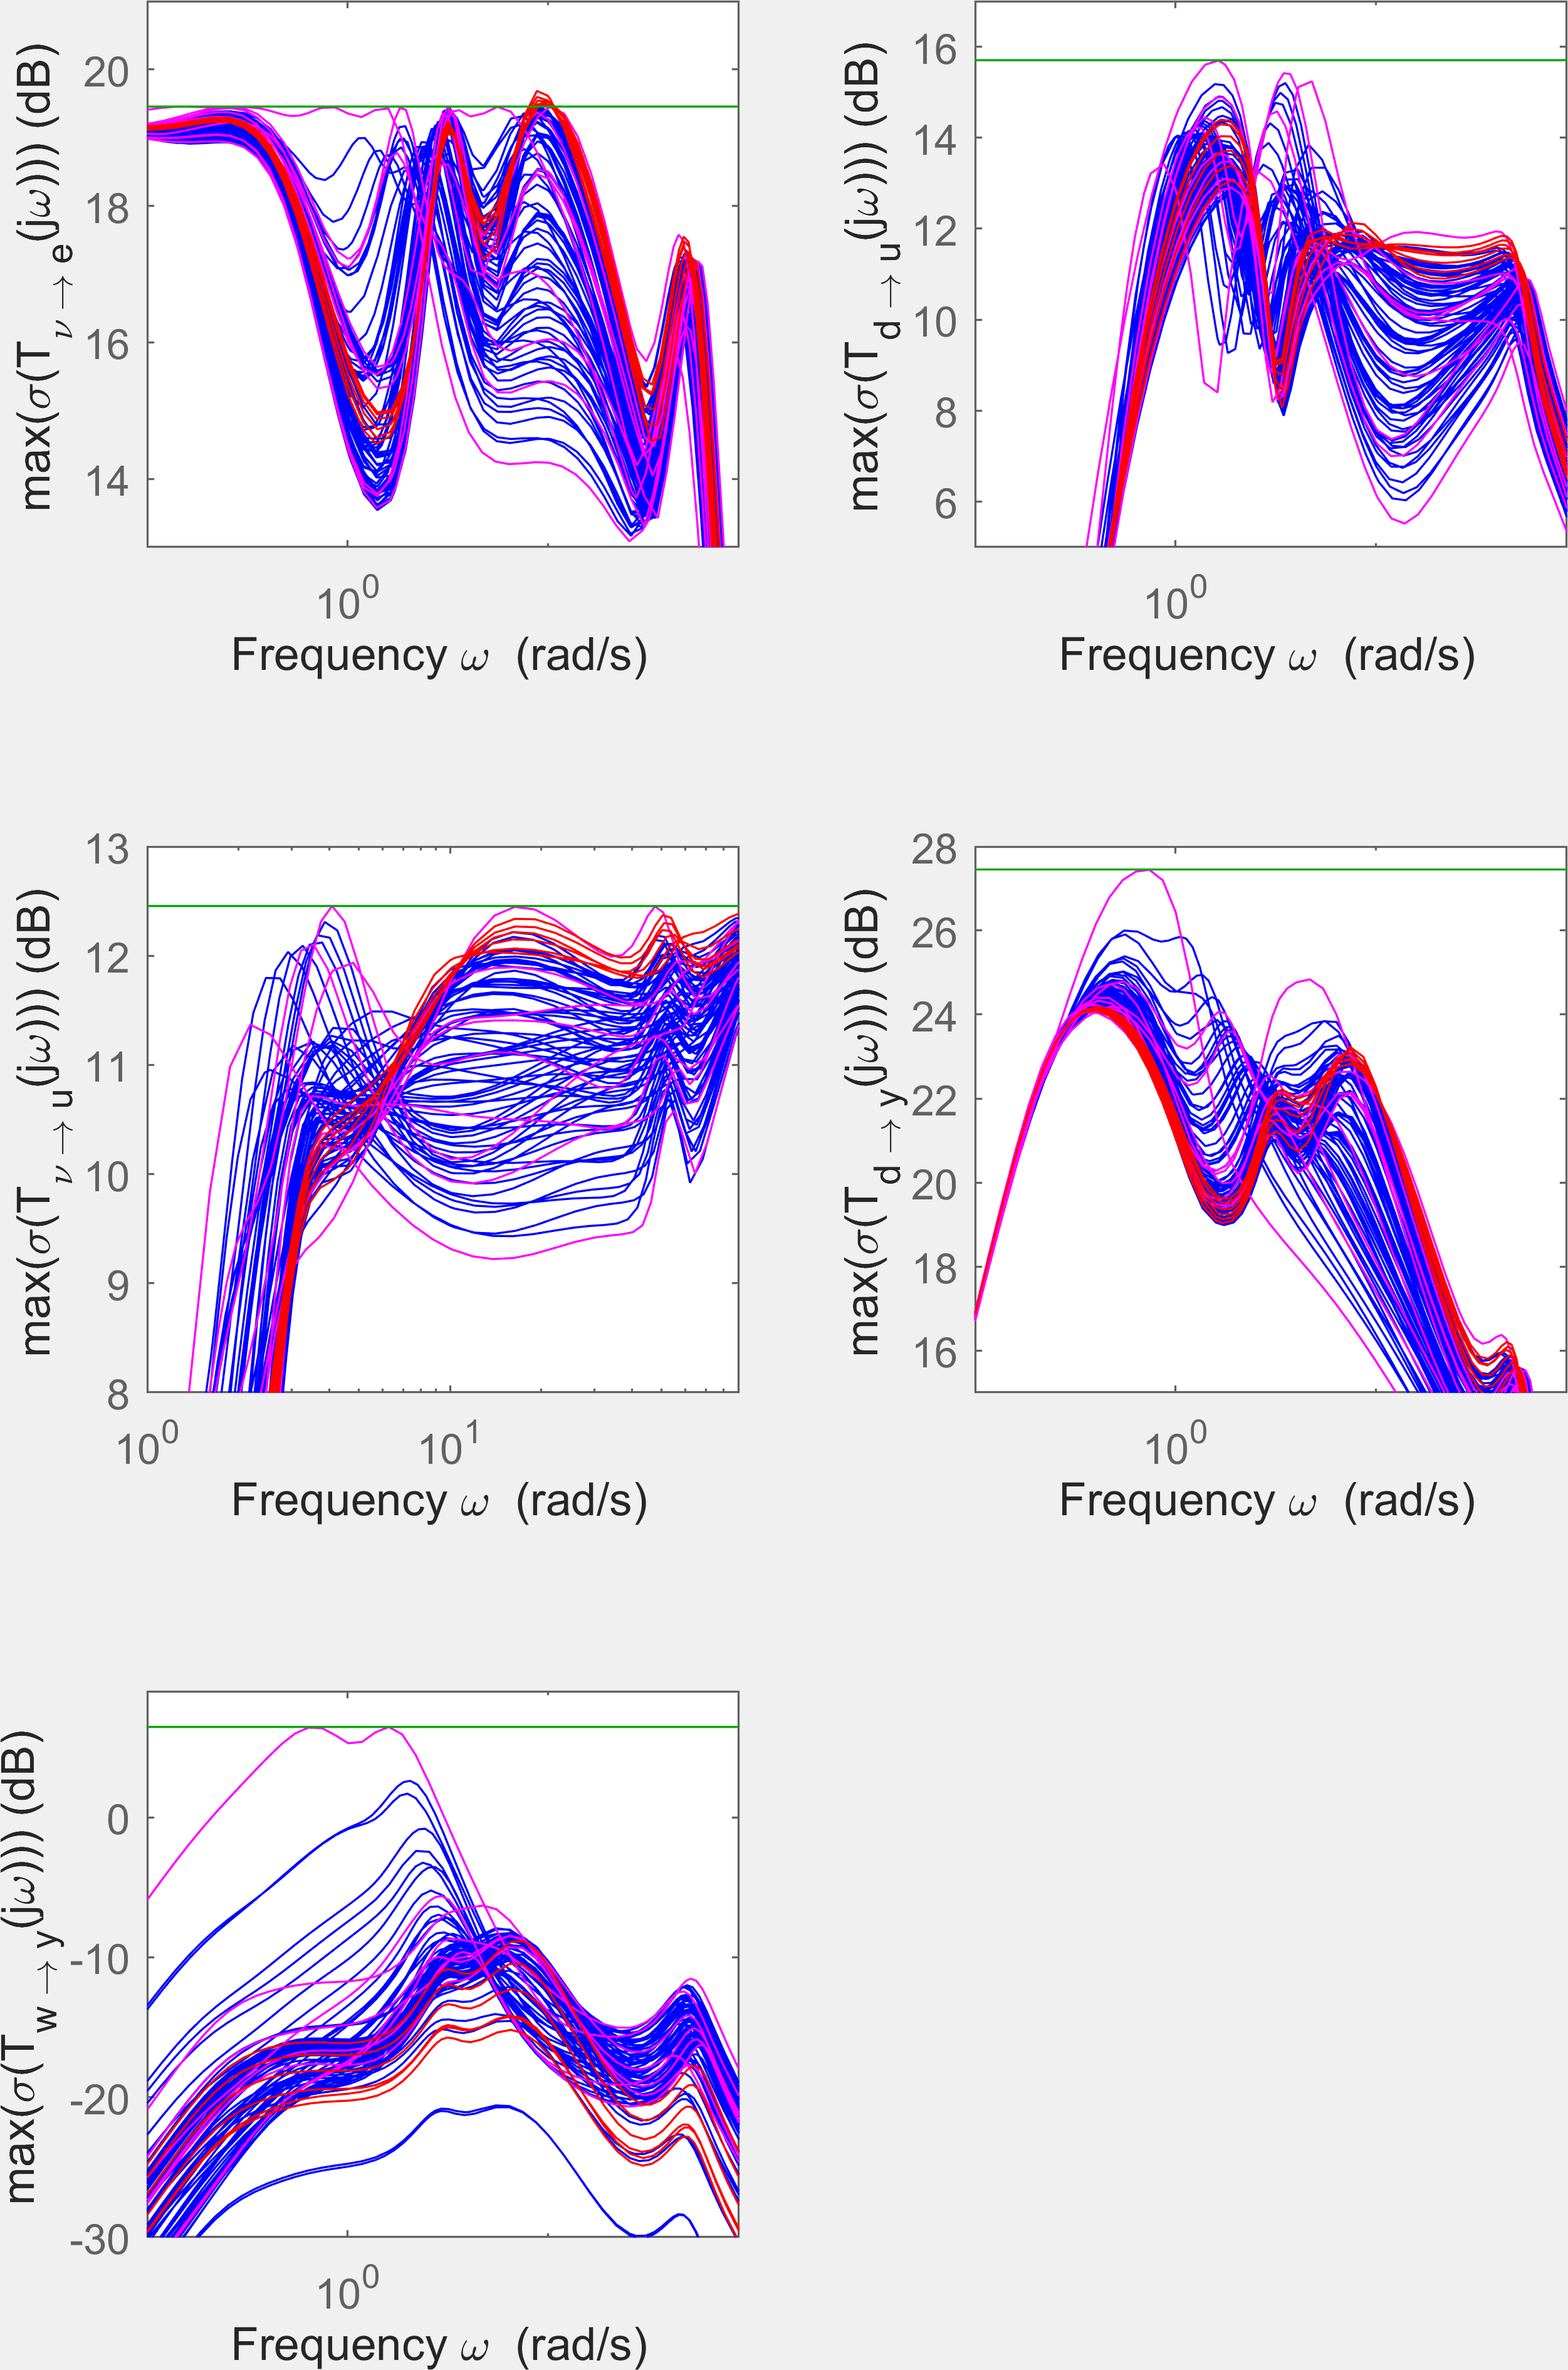
\includegraphics[trim=0cm 0cm 0cm 0cm,clip,width=0.6\columnwidth]{figures/transferts_tcst.png}
    \caption{Diagrammes des valeurs singulières des fonctions de transfert dans \eqref{eq:validation_step}, à la première itération de l'algorithme~\ref{alg:iterativeOptimisation}.}
    \label{fig:transferts_tcst}
\end{figure}
 

\begin{figure}[ht!]
    \centering
    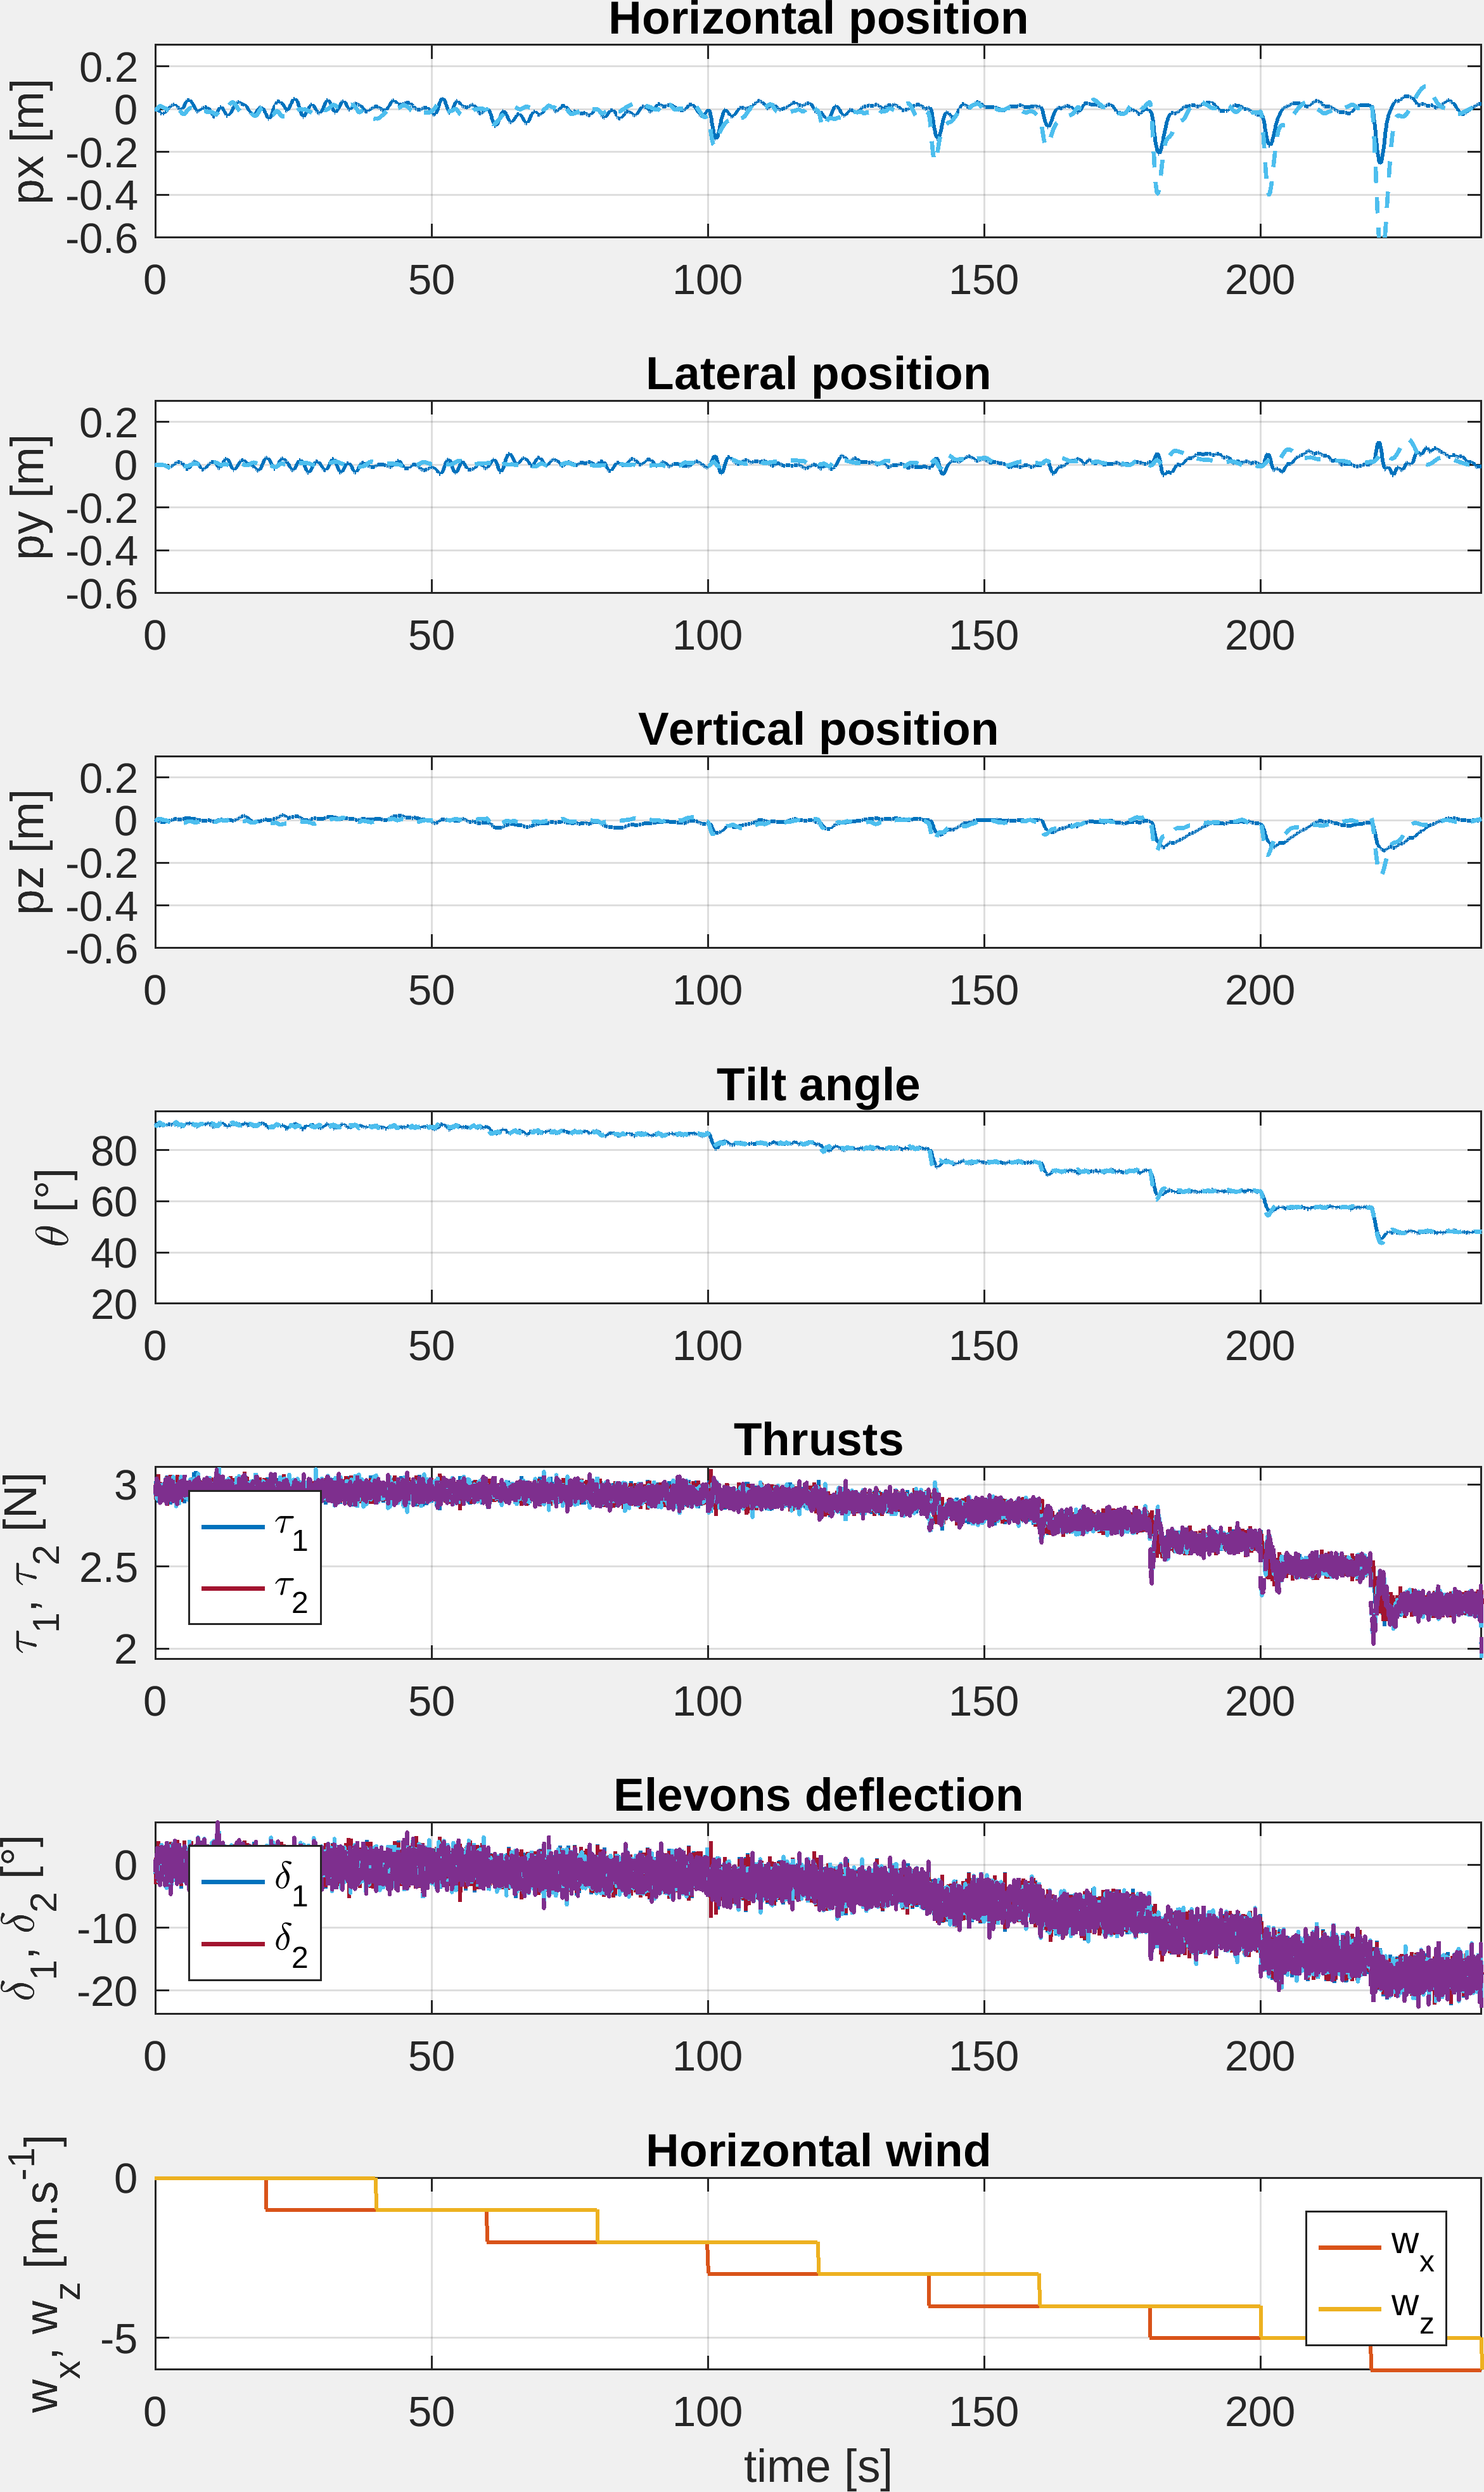
\includegraphics[trim=0cm 0cm 0cm 0cm,clip,width=0.6\columnwidth]{figures/sim_systune_lpv_noise.png}
    \caption{Simulation du modèle non linéaire \eqref{eq:dyna_orig} (ligne continue) et du modèle linéarisé \eqref{eq:lpv_linearisation} (ligne en pointillé) avec des incréments de vent constants croissants, le contrôleur étant réglé à l'aide de l'optimisation multimodèle de l'algorithme~\ref{alg:iterativeOptimisation} dans la section~\ref{sec:h_inf6DOF_multi}.}
    \label{fig:SimSytuneStruct_lpv}
\end{figure}

Avec le réglage indiqué dans \eqref{eq:gain_selection}, tel qu'il est obtenu avec l'Algorithme~\ref{alg:iterativeOptimisation}, nous présentons dans la Figure~\ref{fig:SimSytuneStruct_lpv} des résultats de simulation similaires à ceux déjà présentés dans la Figure.~\ref{fig:SimSytuneStruct_zero} pour la méthode de réglage sans vent discutée dans la Section~\ref{sec:zerowind}. Une fois de plus, nous simulons à la fois le modèle non linéaire \eqref{eq:dyna_orig} (lignes pleines) et le modèle linéarisé \eqref{eq:lpv_linearisation} (ligne en pointillé). 

Par rapport à la Fig.~\ref{fig:SimSytuneStruct_zero}, les simulations de la Figure~\ref{fig:SimSytuneStruct_lpv} montrent que le réglage du contrôleur basé sur les Théorèmes~\ref{thm:eqs} et~\ref{th:lin} résout les problèmes d'instabilité et parvient à stabiliser le vol stationnaire dans tous les scénarios de vent considérés. Nous notons également que la Figure.~\ref{fig:SimSytuneStruct_lpv} montre une action plus agressive. En effet, l'entrée de contrôle $u$ (à la fois la poussée et les déflexions) est plus affectée par le bruit de mesure.

L'efficacité du schéma de contrôle réglé sur la base de l'Algorithme~\ref{alg:iterativeOptimisation} est également confirmée par les résultats expérimentaux présentés dans la section suivante.

\section{Rafale de vent}

Dans le chapitre \ref{sec:perturbation}, nous avons présenté des modèles de perturbation représentant une modélisation d'une rafale de vent. Nous allons les utiliser pour évaluer la réponse du drone face à cette perturbation. 


Nous avons appliqué un vent horizontal $w_x$ avec trois valeurs moyennes $w_{m} \in {0,3,6}\SI{}{\meter\per\second}$ et avec les caractéristiques suivantes pour la fonction "Chapeau mexicain" $A_g=\SI{-5}{\meter\per\second}$, $f_g = \frac{1}{T_g} = \SI{0.2}{\Hz}$ soit une période $T_g$ de 5 secondes. Les résultats sont visibles sur la figure \ref{fig:sim_mex0_2}.
\begin{figure}[ht!]
    \centering
    \resizebox{.99\textwidth}{!}{%
    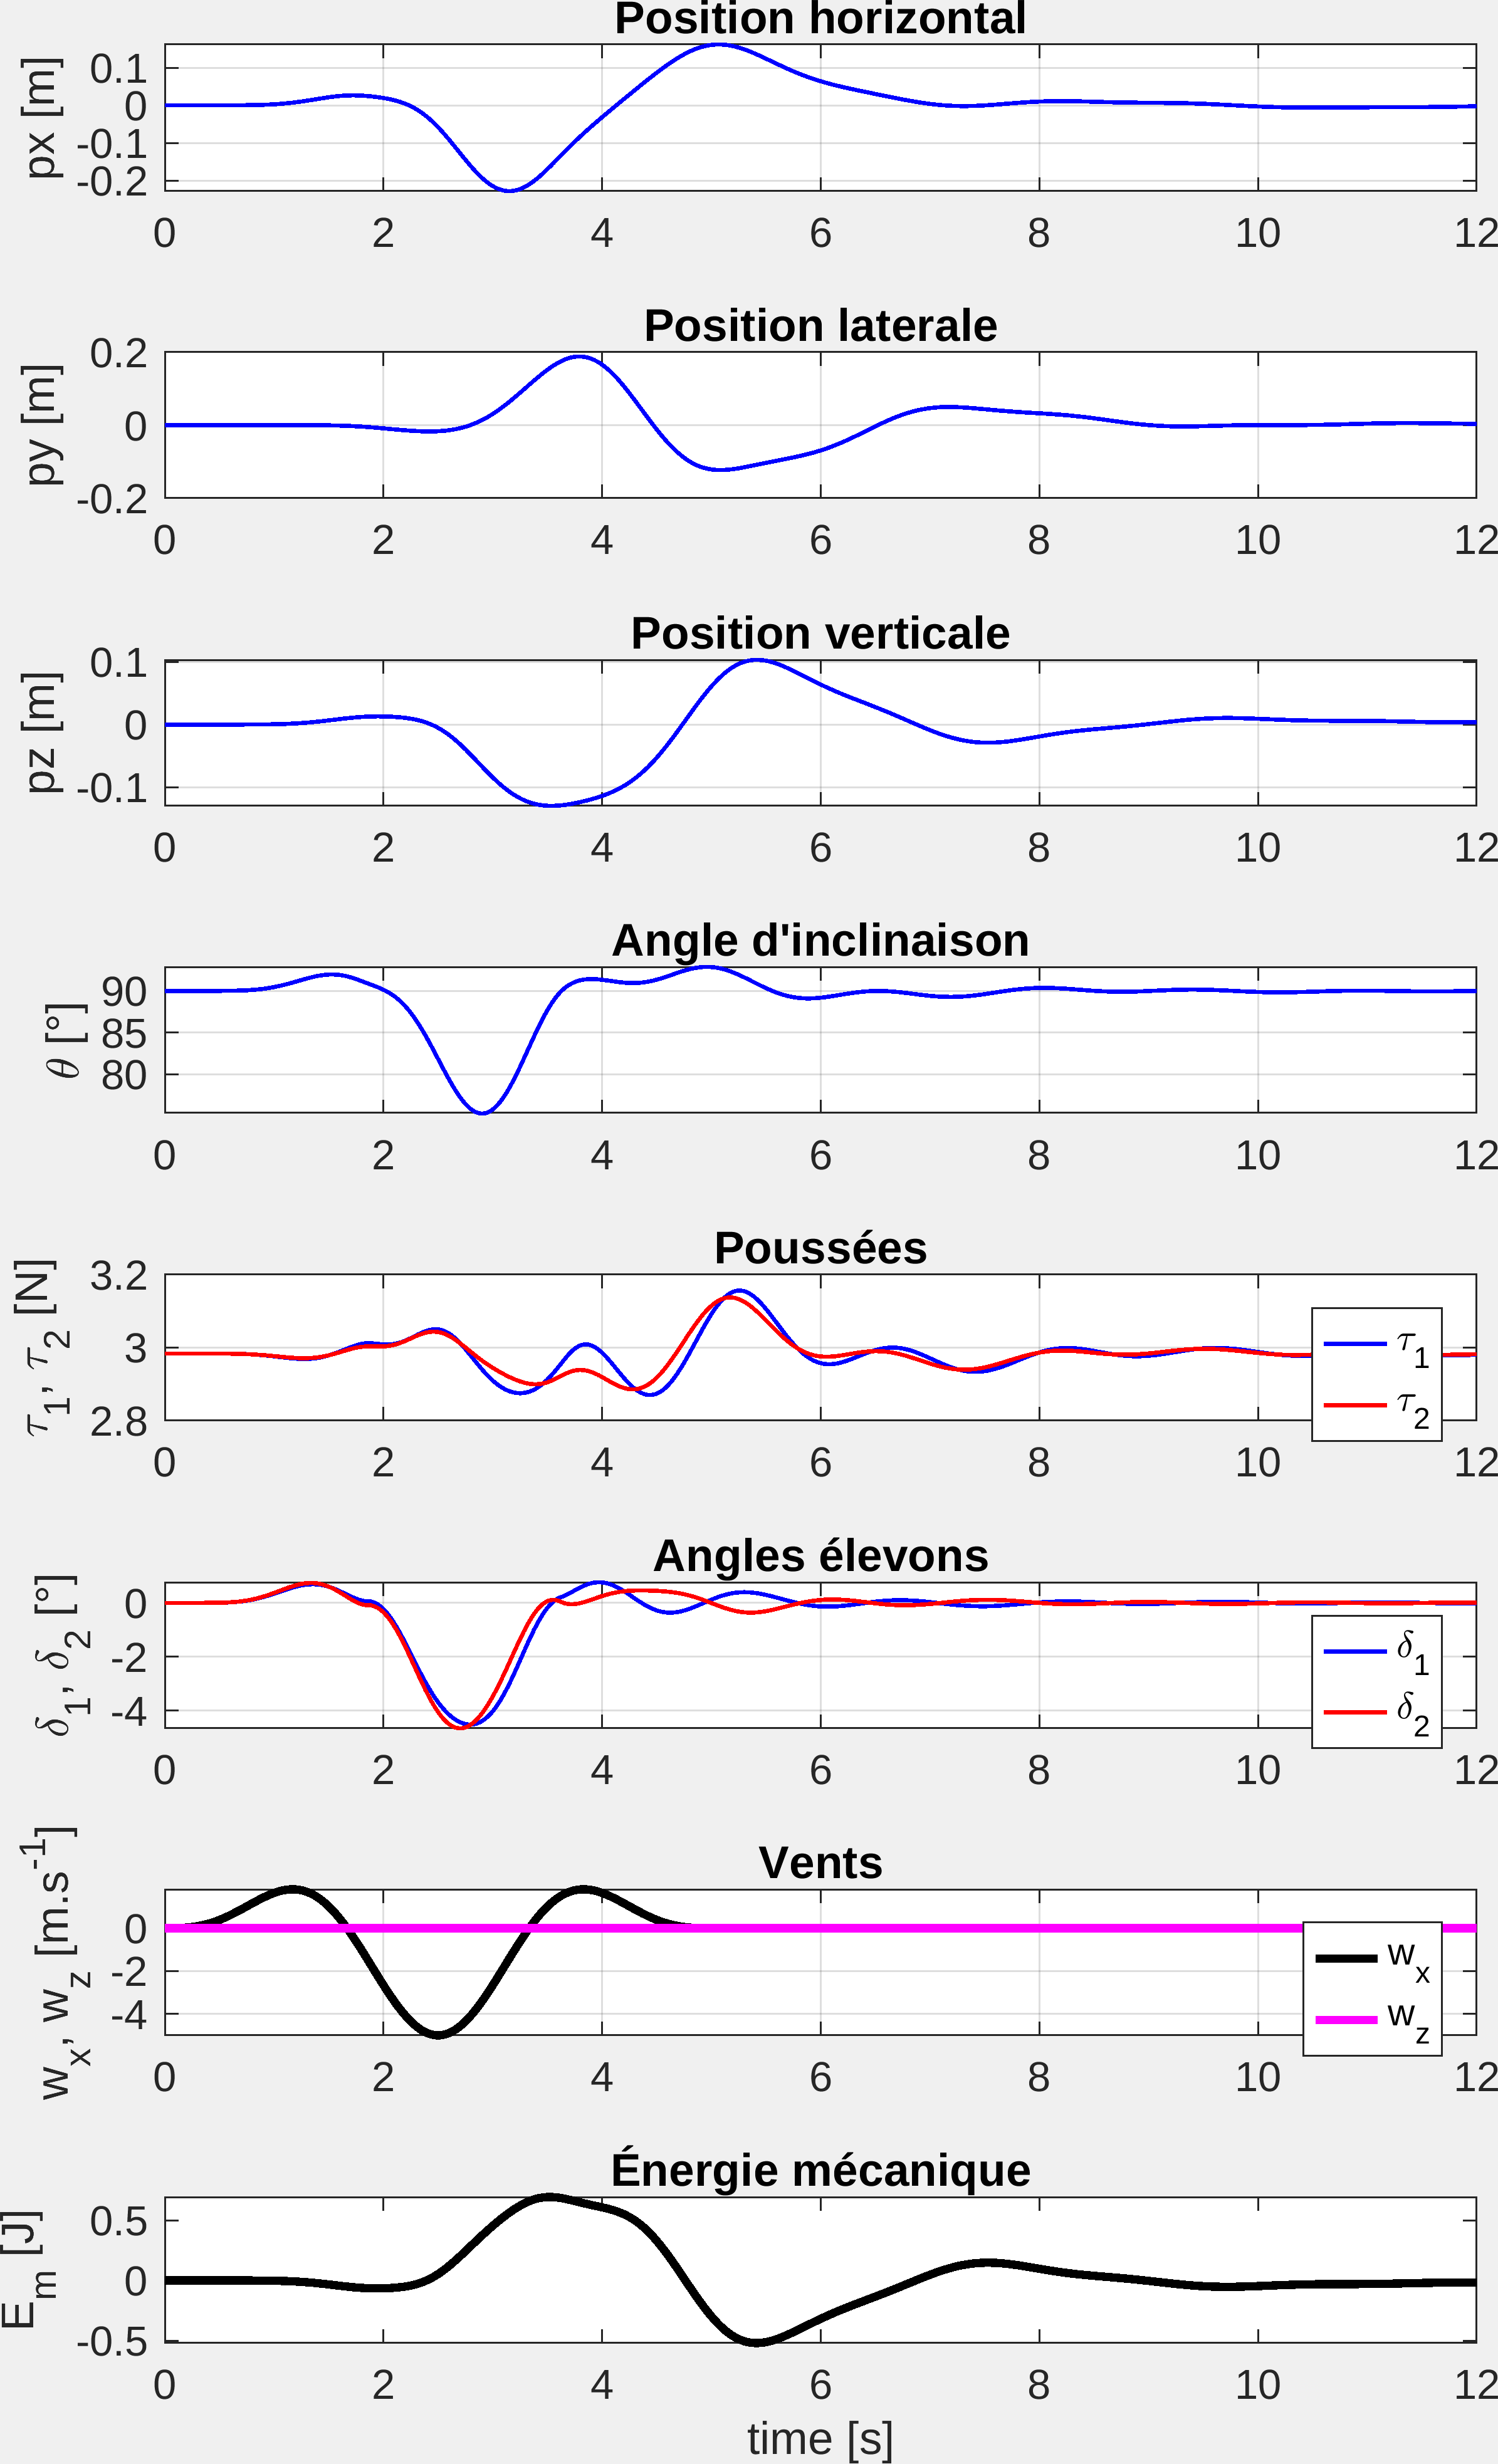
\includegraphics[width=0.33\textwidth]{figures/sim_mex_hat5msT5.png}
    \quad
    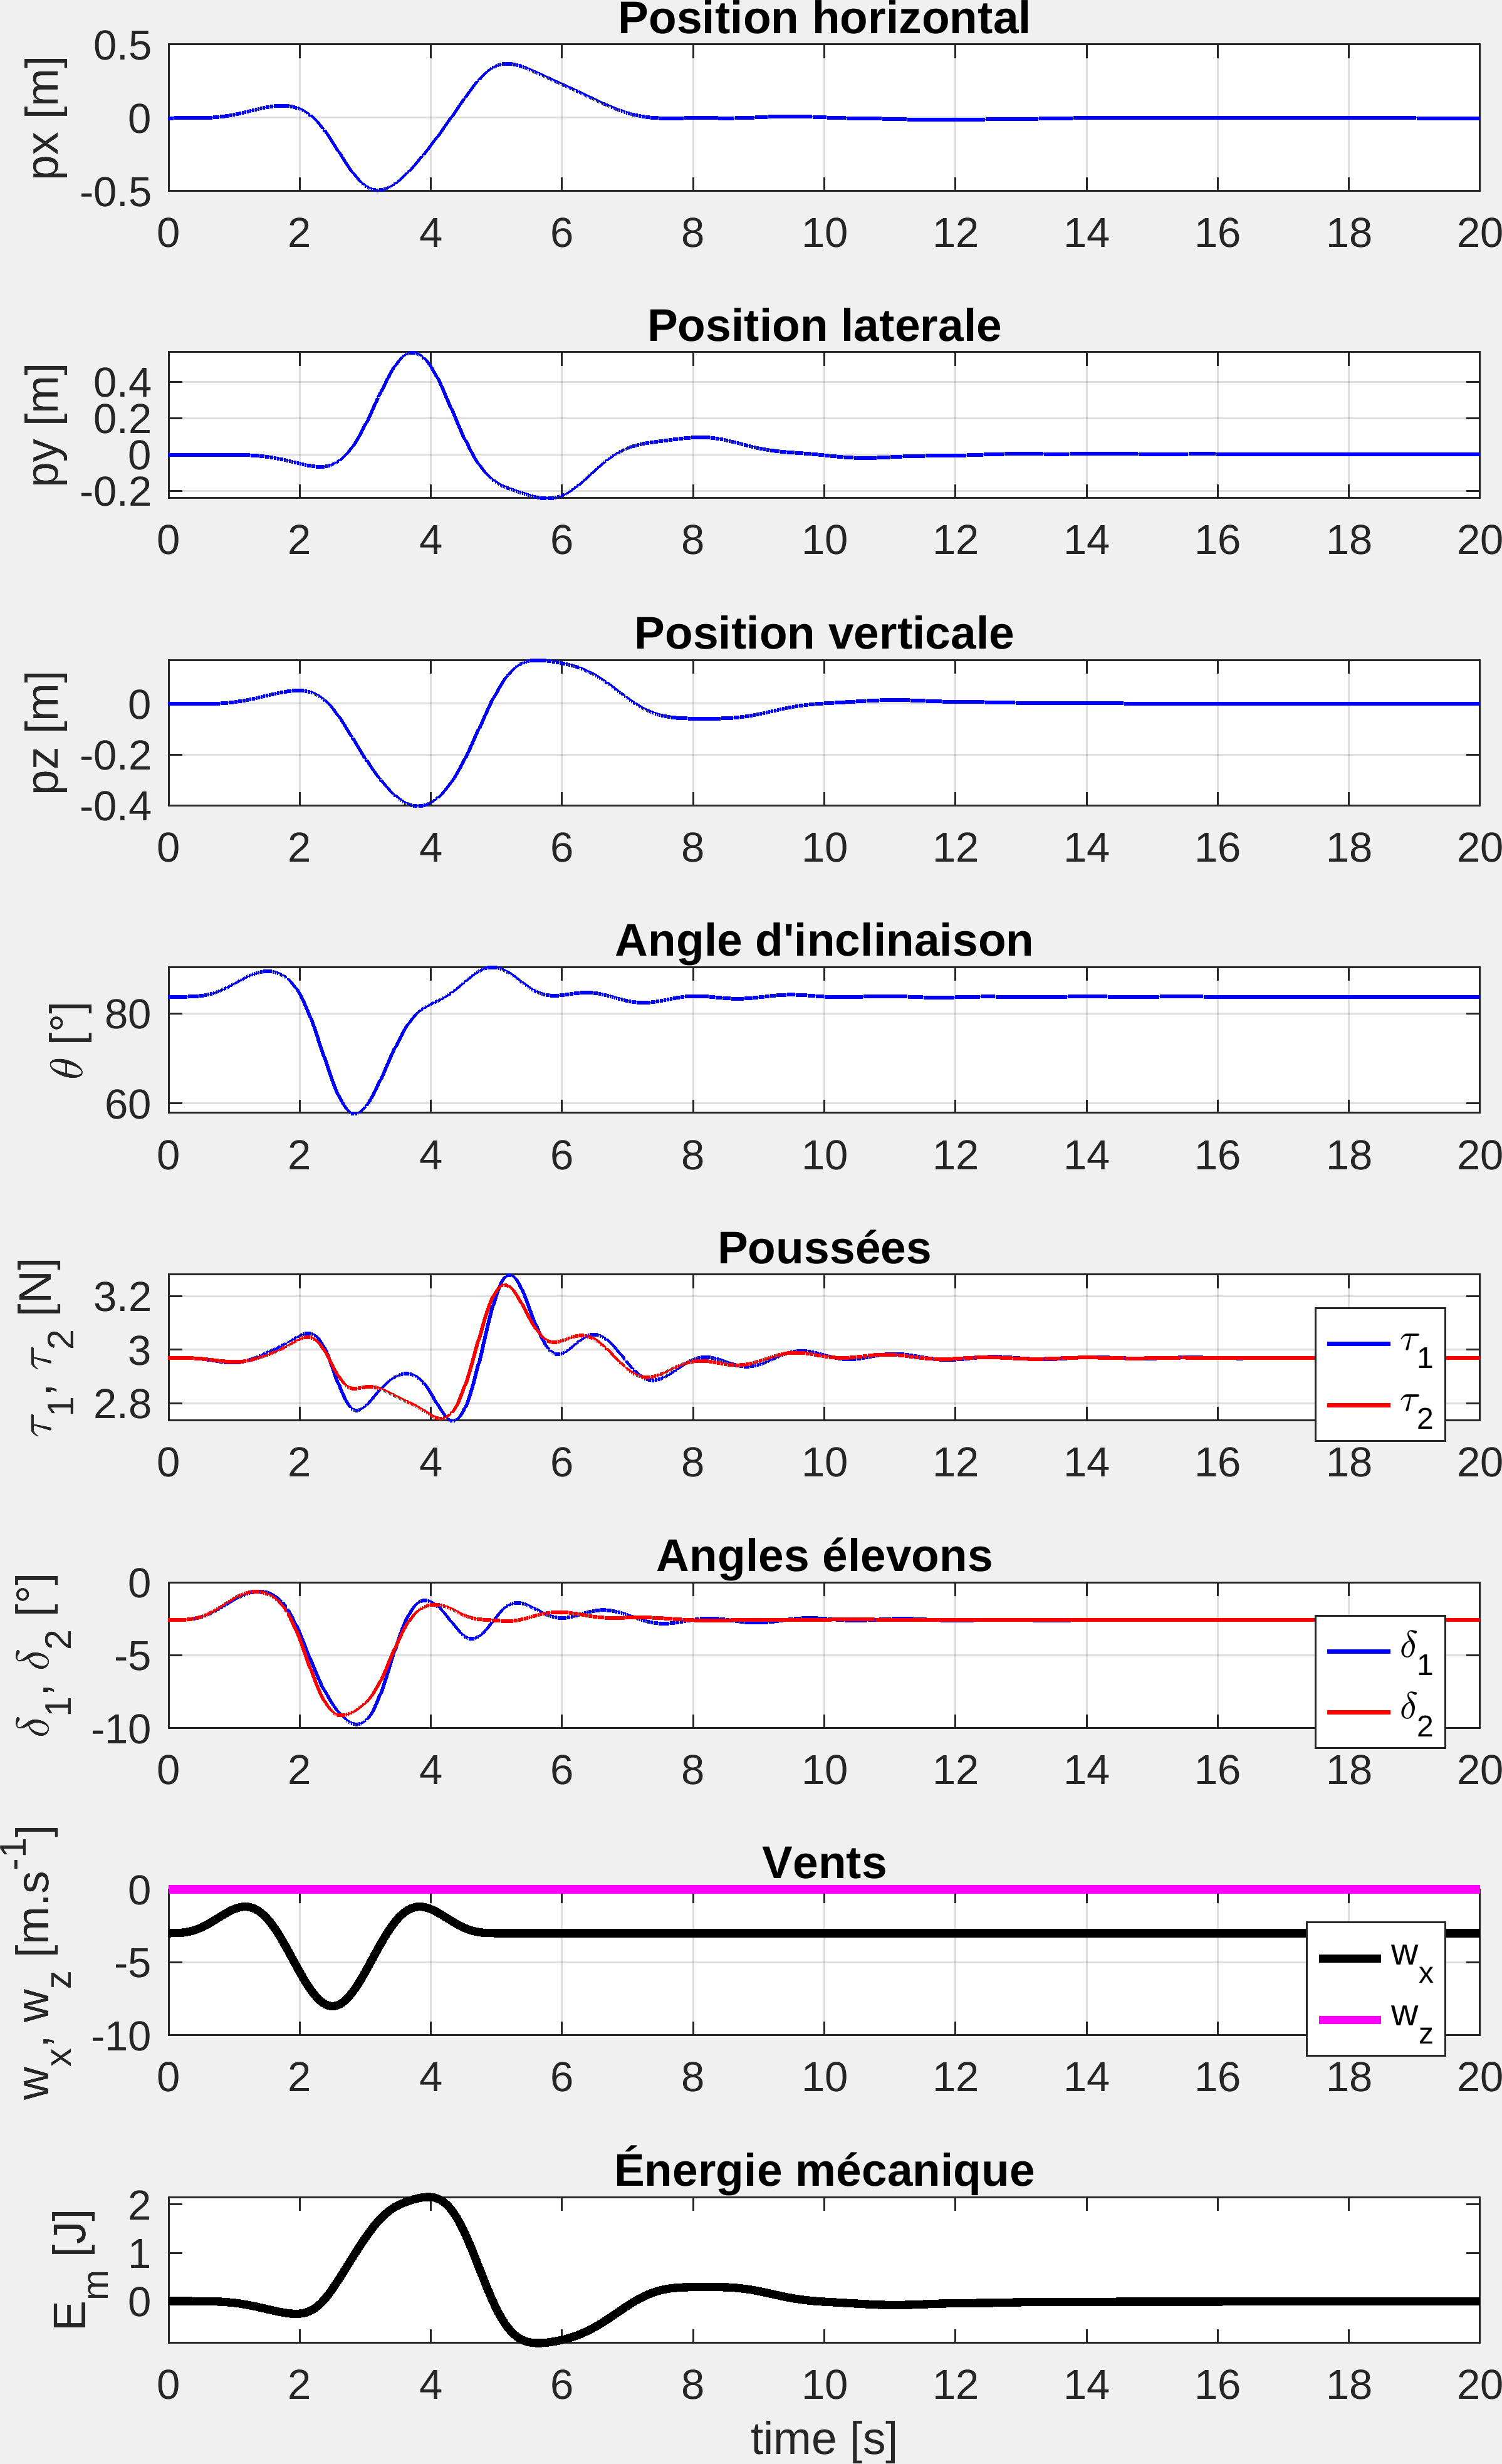
\includegraphics[width=0.33\textwidth]{figures/sim_mex_hat8msT5.png}
    \quad
    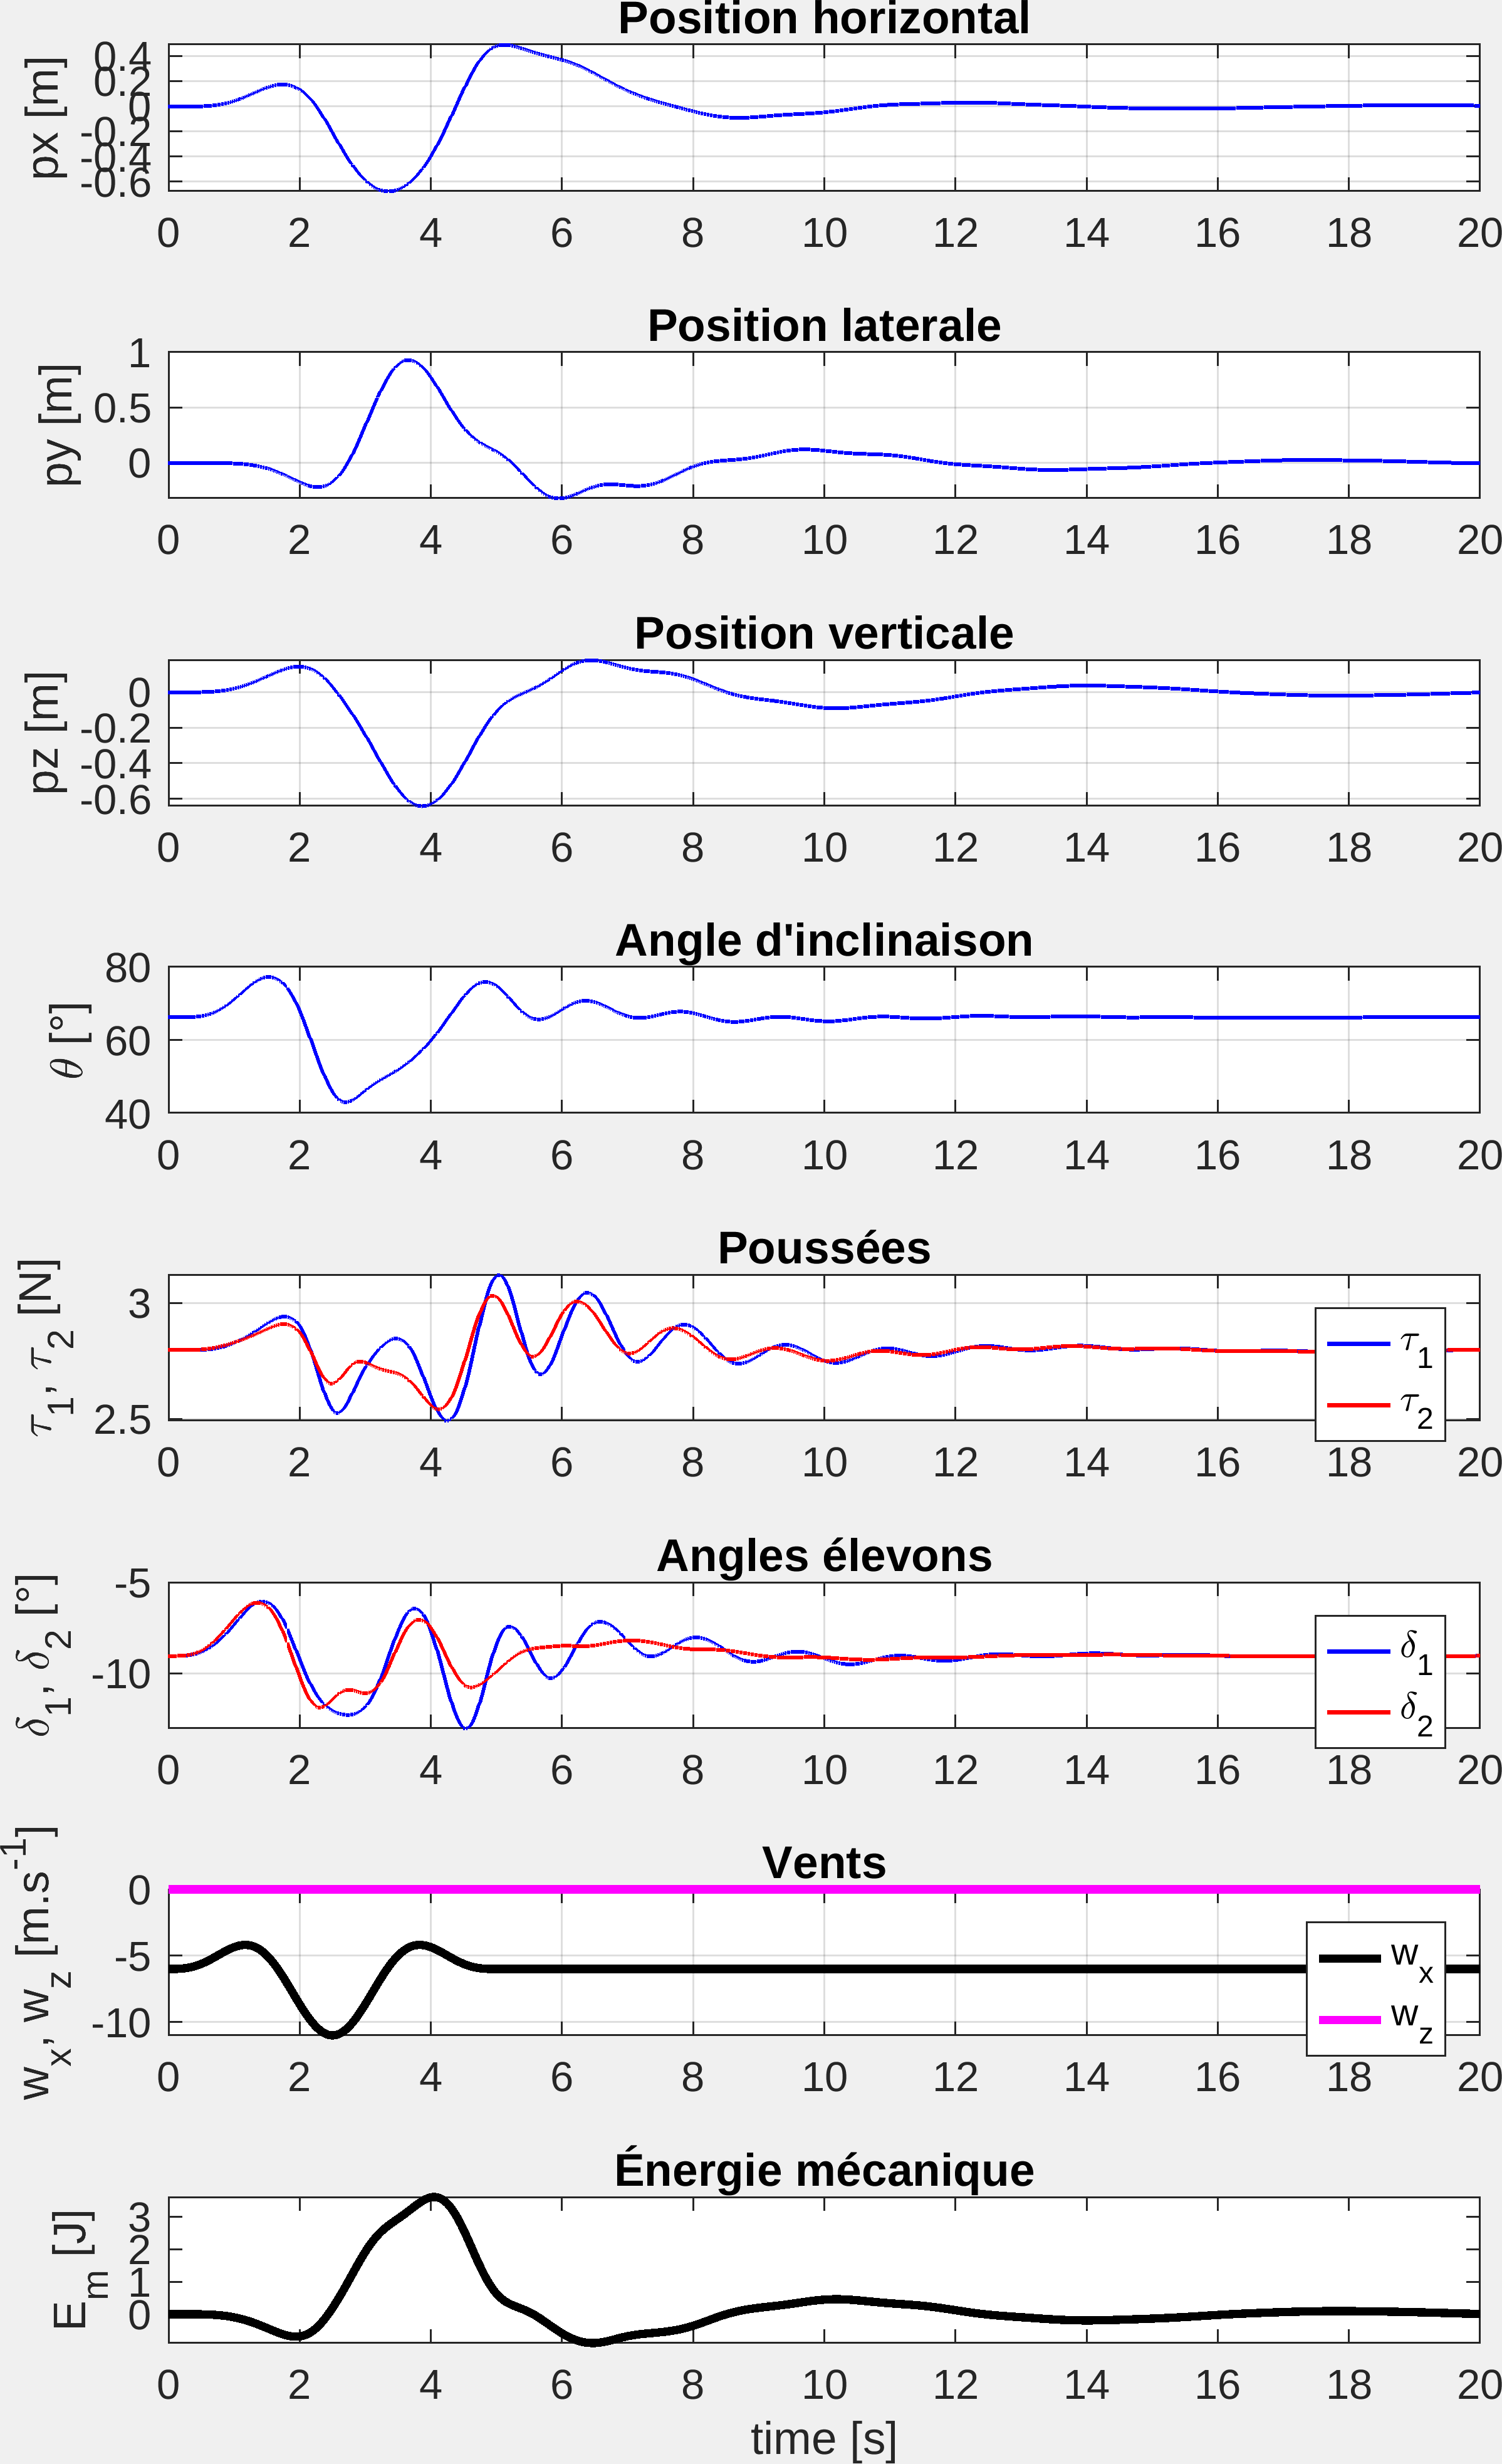
\includegraphics[width=0.33\textwidth]{figures/sim_mex_hat11msT5.png}
    }
    \caption{Simulation du modèle non linéaire \eqref{eq:dyna_orig} face à une perturbation "Chapeau mexicain" \eqref{eq:mex} avec $f_g = \SI{0.2}{\Hz}$.}
    \label{fig:sim_mex0_2}
\end{figure}


Nous avons aussi réalisé une simulation similaire à la précédente avec une fréquence égale à $f_g = \SI{1.2}{\Hz}$ soit une période $T_g$ de 0.83 seconde. Cette valeur est utilisée dans \cite{Gillebaart2014} pour représenter une rafale. Les résultats sont visibles sur la figure \ref{fig:sim_mex1_2}.
\begin{figure}[h]
    \centering
    \resizebox{.99\textwidth}{!}{%
    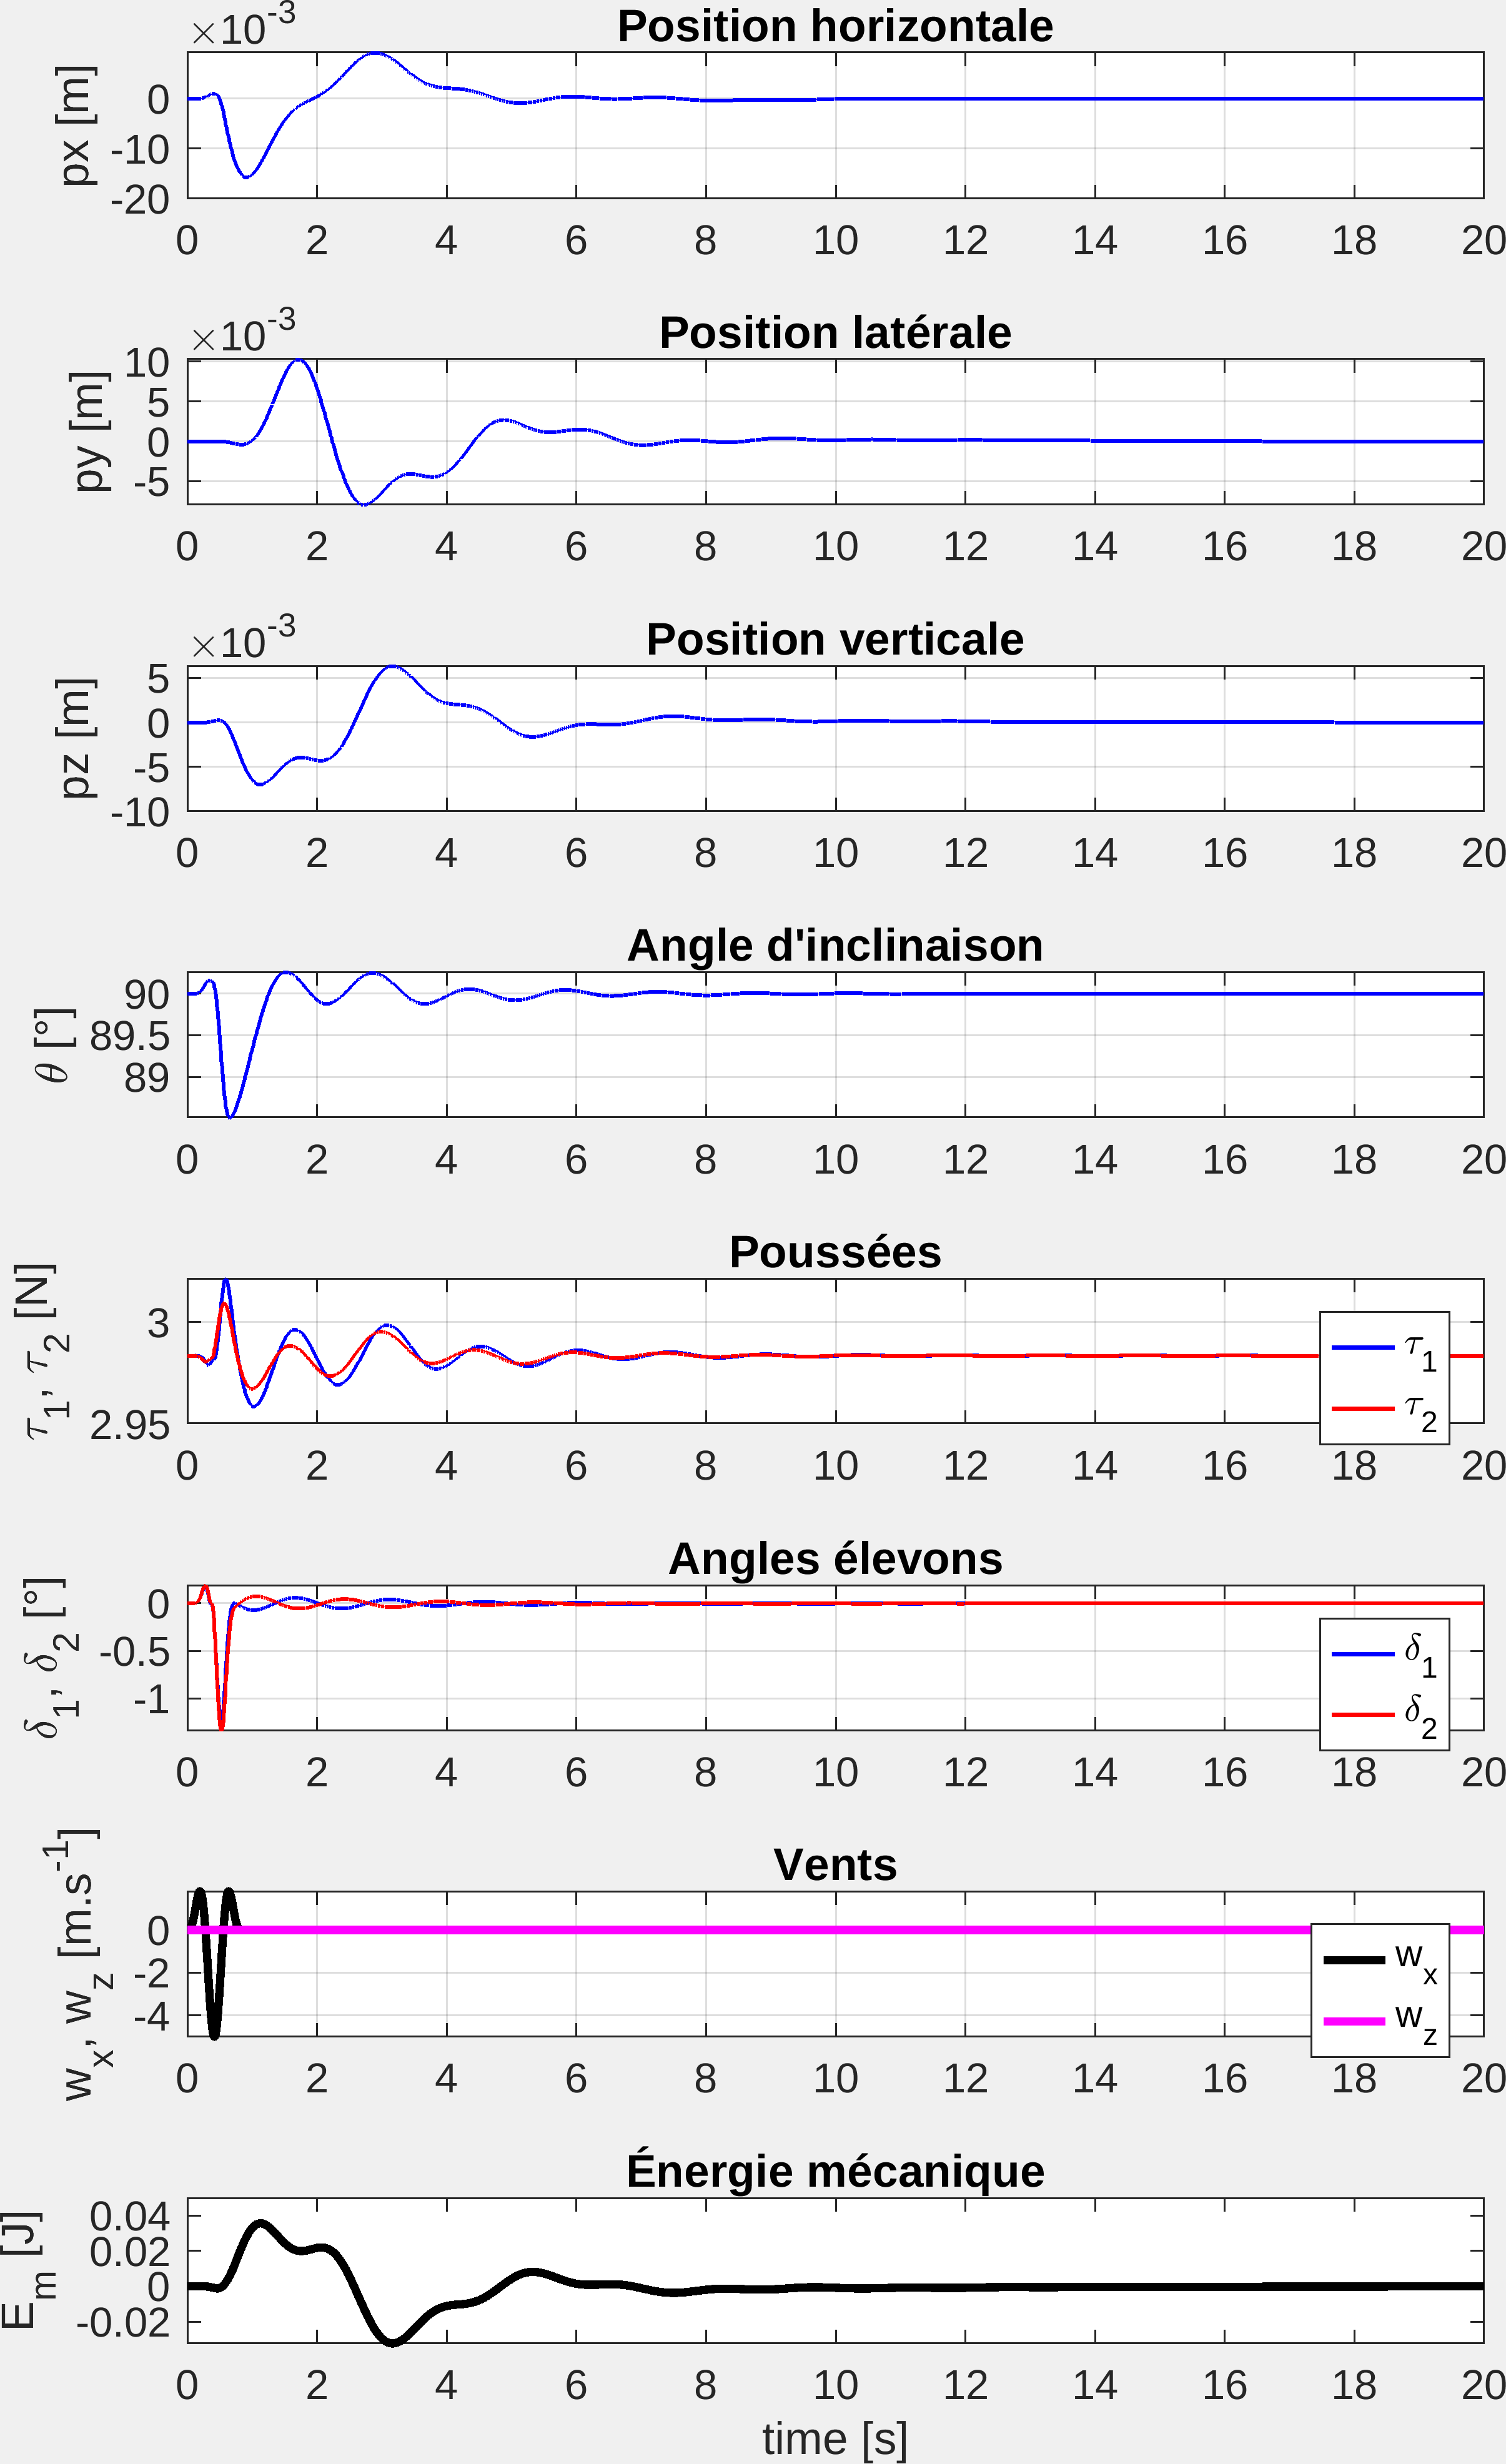
\includegraphics[width=0.33\textwidth]{figures/sim_mex_hat5msF1.2.png}
    \quad
    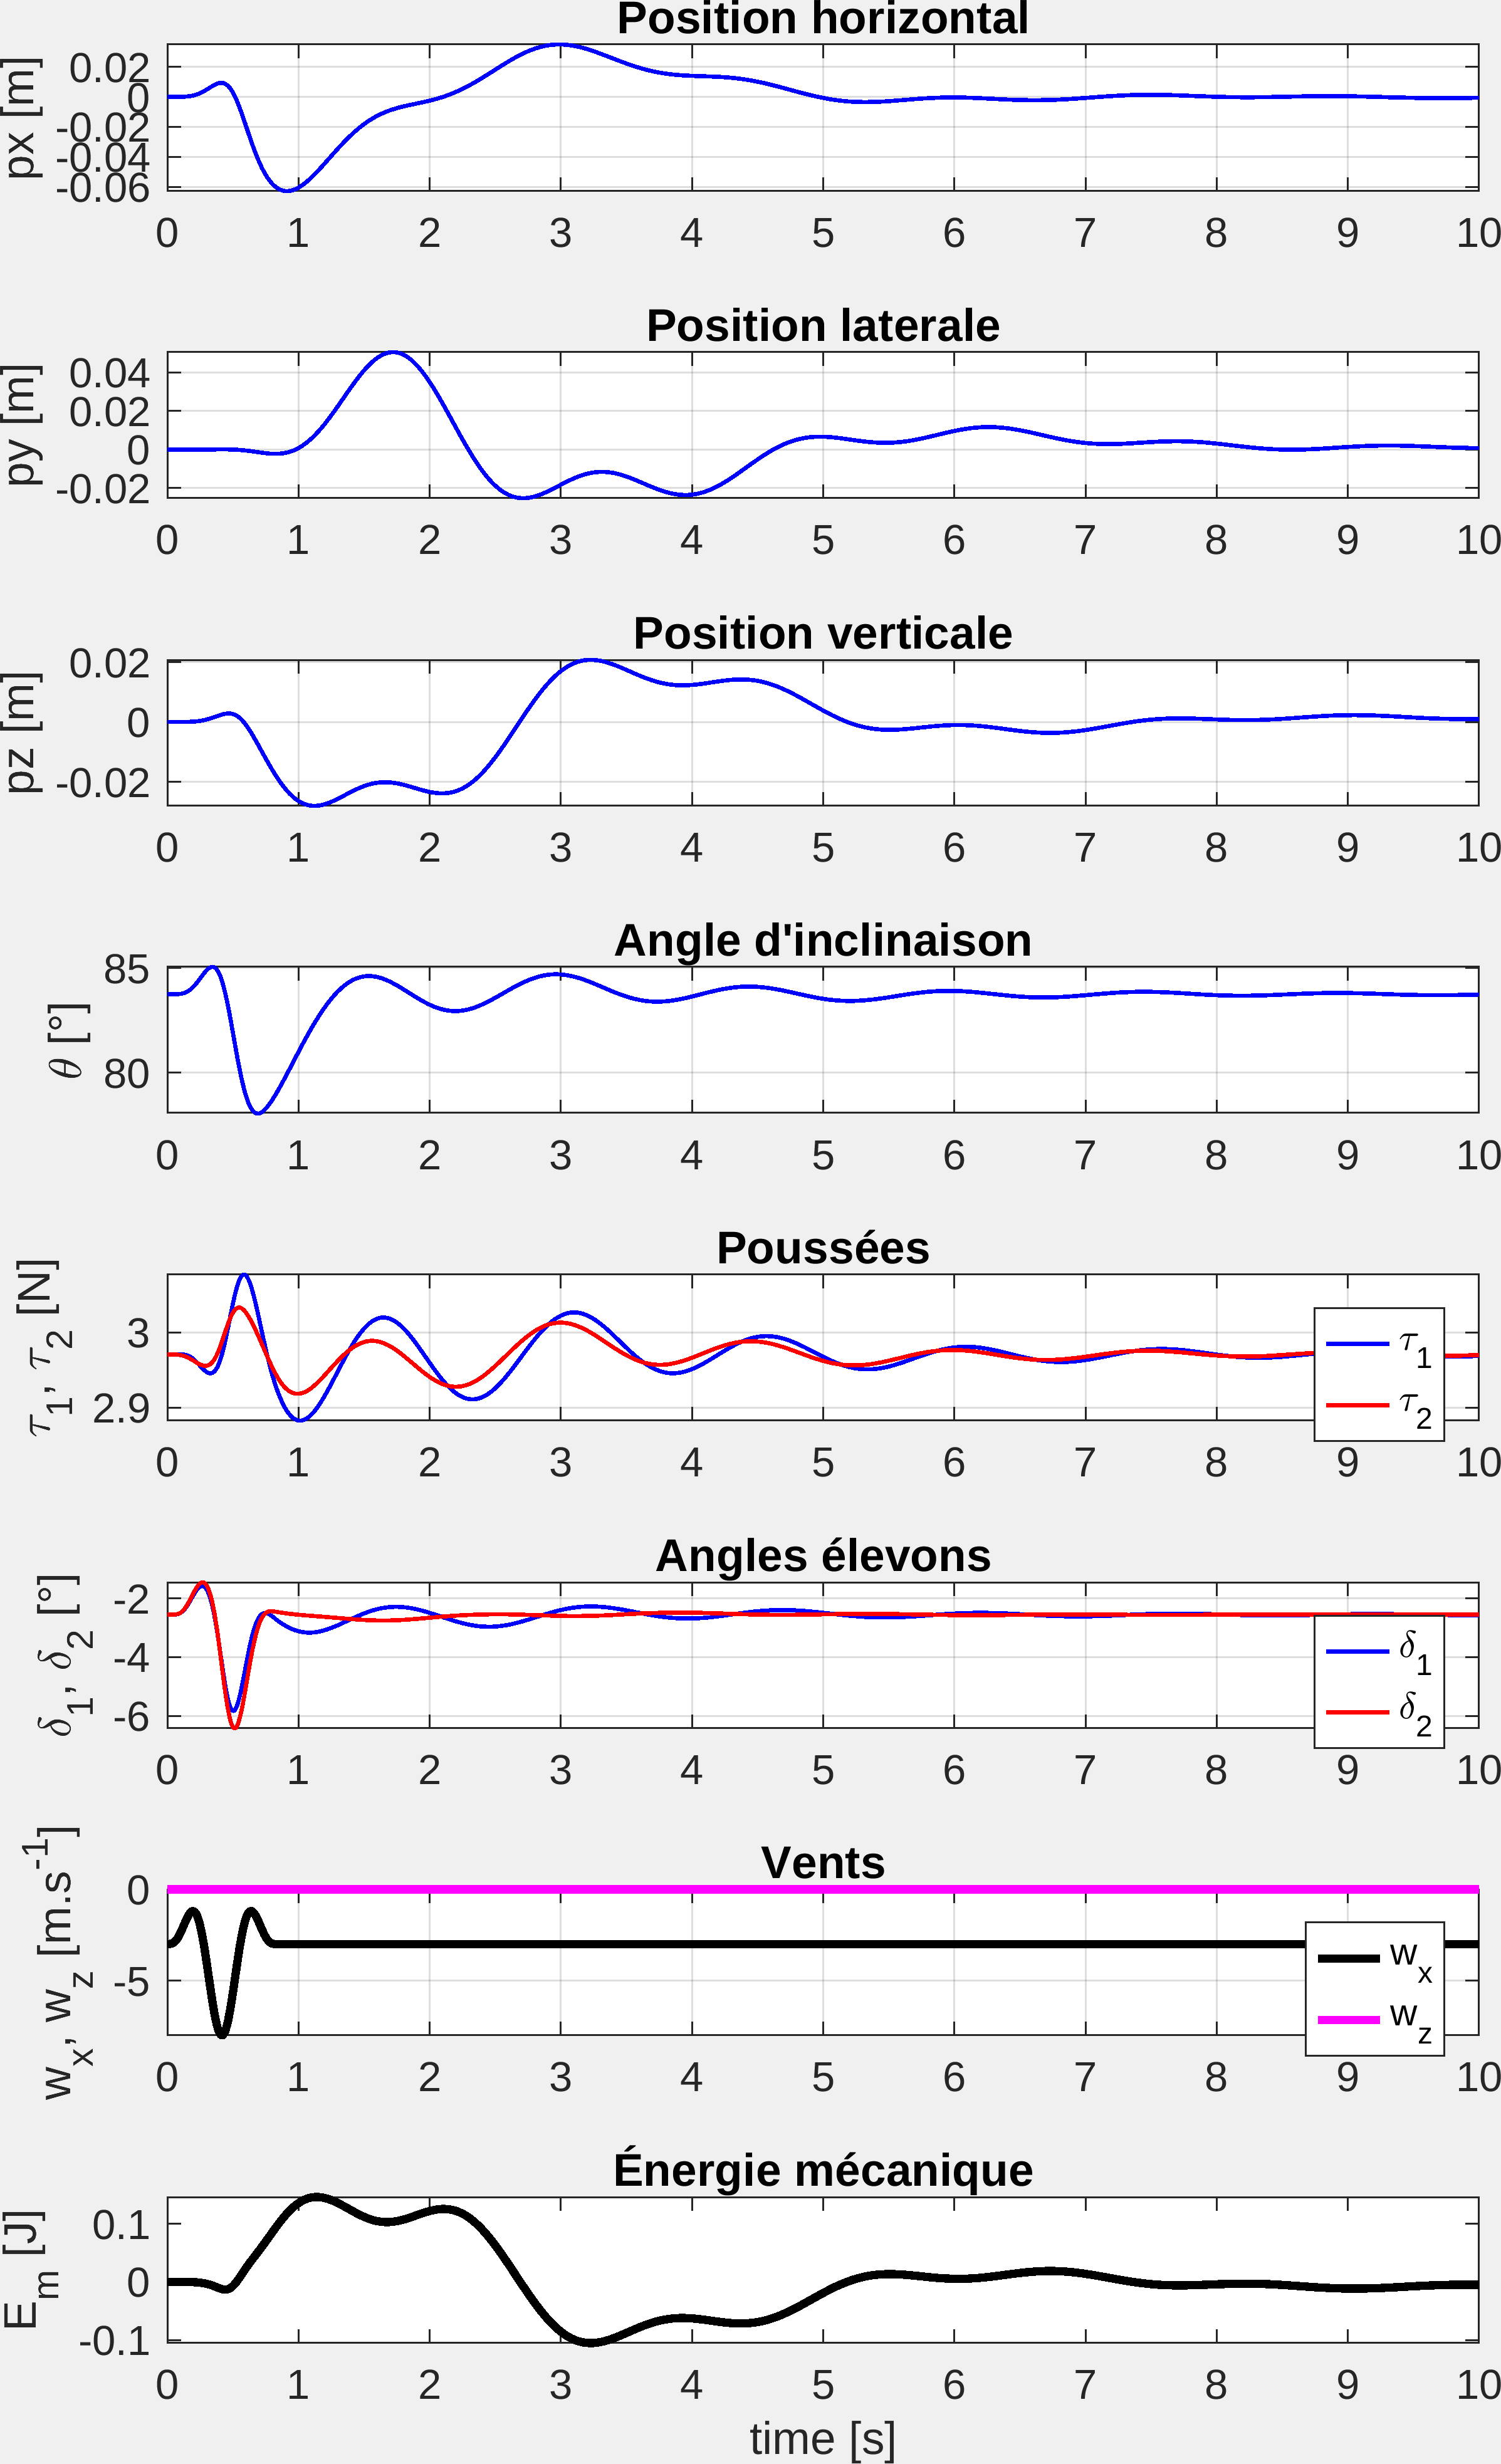
\includegraphics[width=0.33\textwidth]{figures/sim_mex_hat8msF1.2.png}
    \quad
    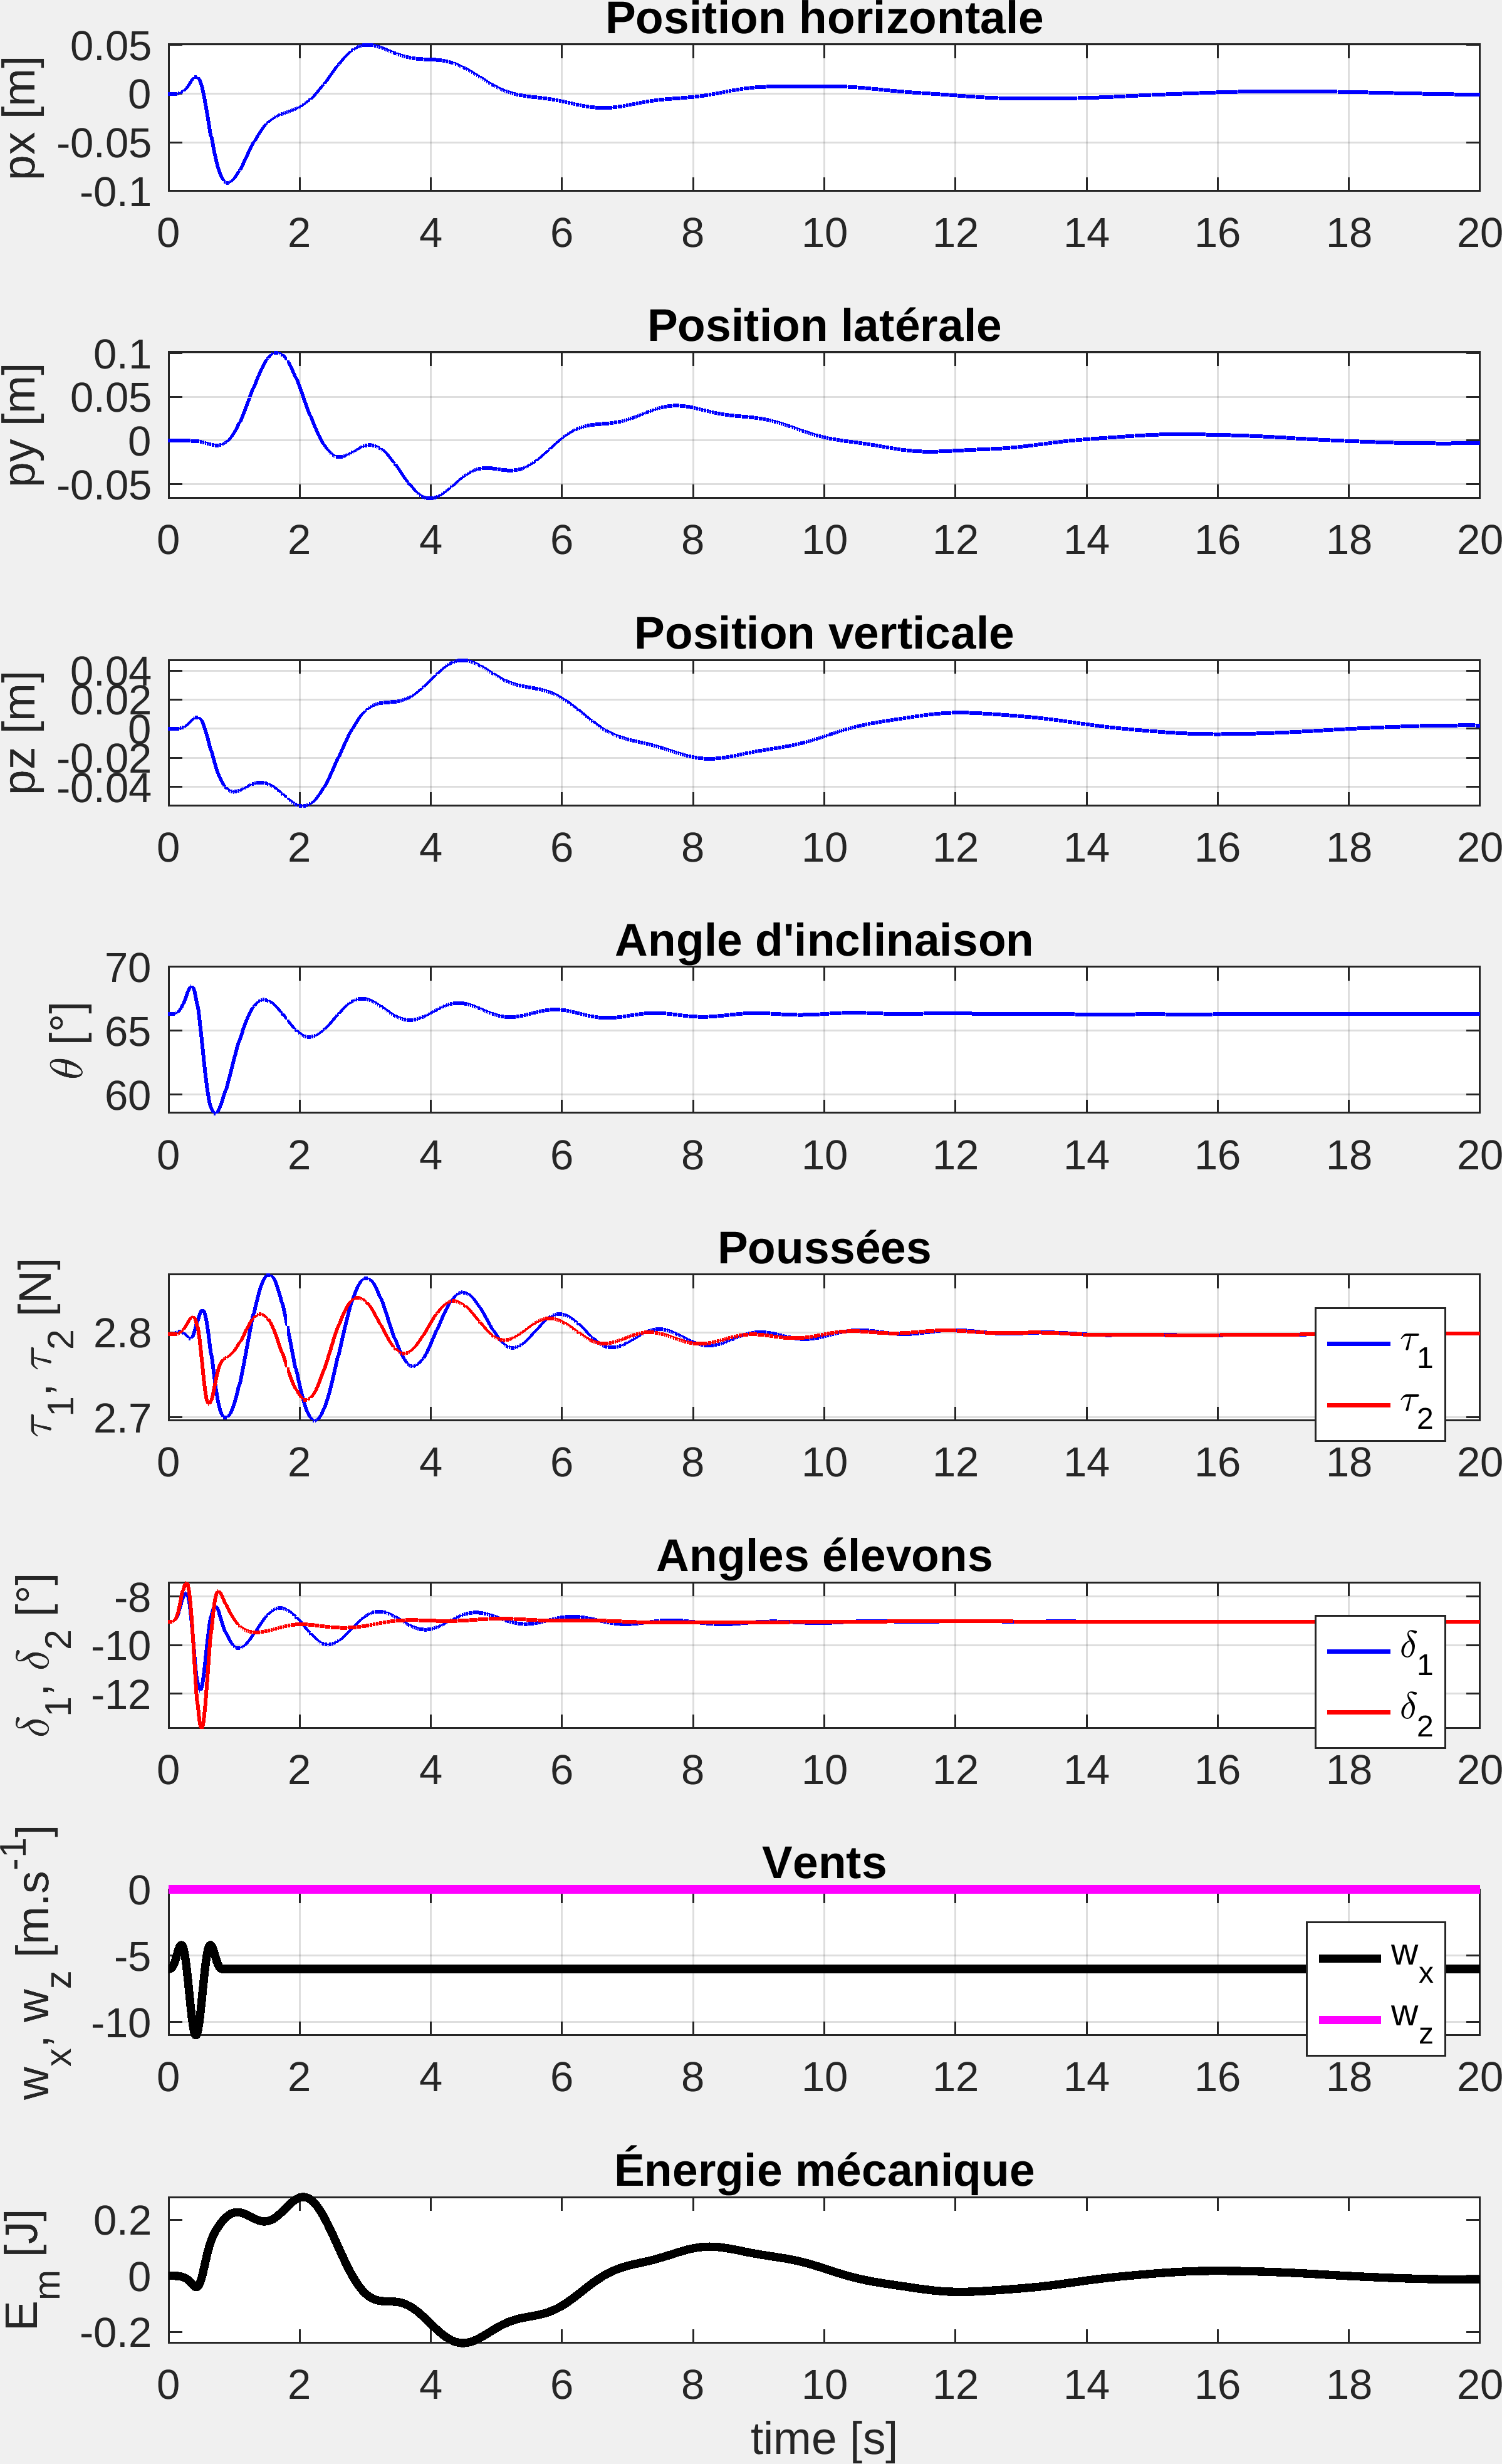
\includegraphics[width=0.33\textwidth]{figures/sim_mex_hat11msF1.2.png}
    }
    \caption{Simulation du modèle non linéaire \eqref{eq:dyna_orig} face à une perturbation "Chapeau mexicain" \eqref{eq:mex} avec $f_g = \SI{1.2}{\Hz}$.}
    \label{fig:sim_mex1_2}
\end{figure}


Enfin nous avons réalisé une simulation avec un vent horizontal $w_x$ avec trois valeurs moyennes $w_{m} \in {0,3,6}\SI{}{\meter\per\second}$ et avec la caractéristique suivante pour la fonction "ondelettes de Morlet" $A_g=\SI{-5}{\meter\per\second}$. Les résultats sont visibles sur la figure \ref{fig:sim_morlet}.

\begin{figure}[h]
    \centering
    \resizebox{.99\textwidth}{!}{%
    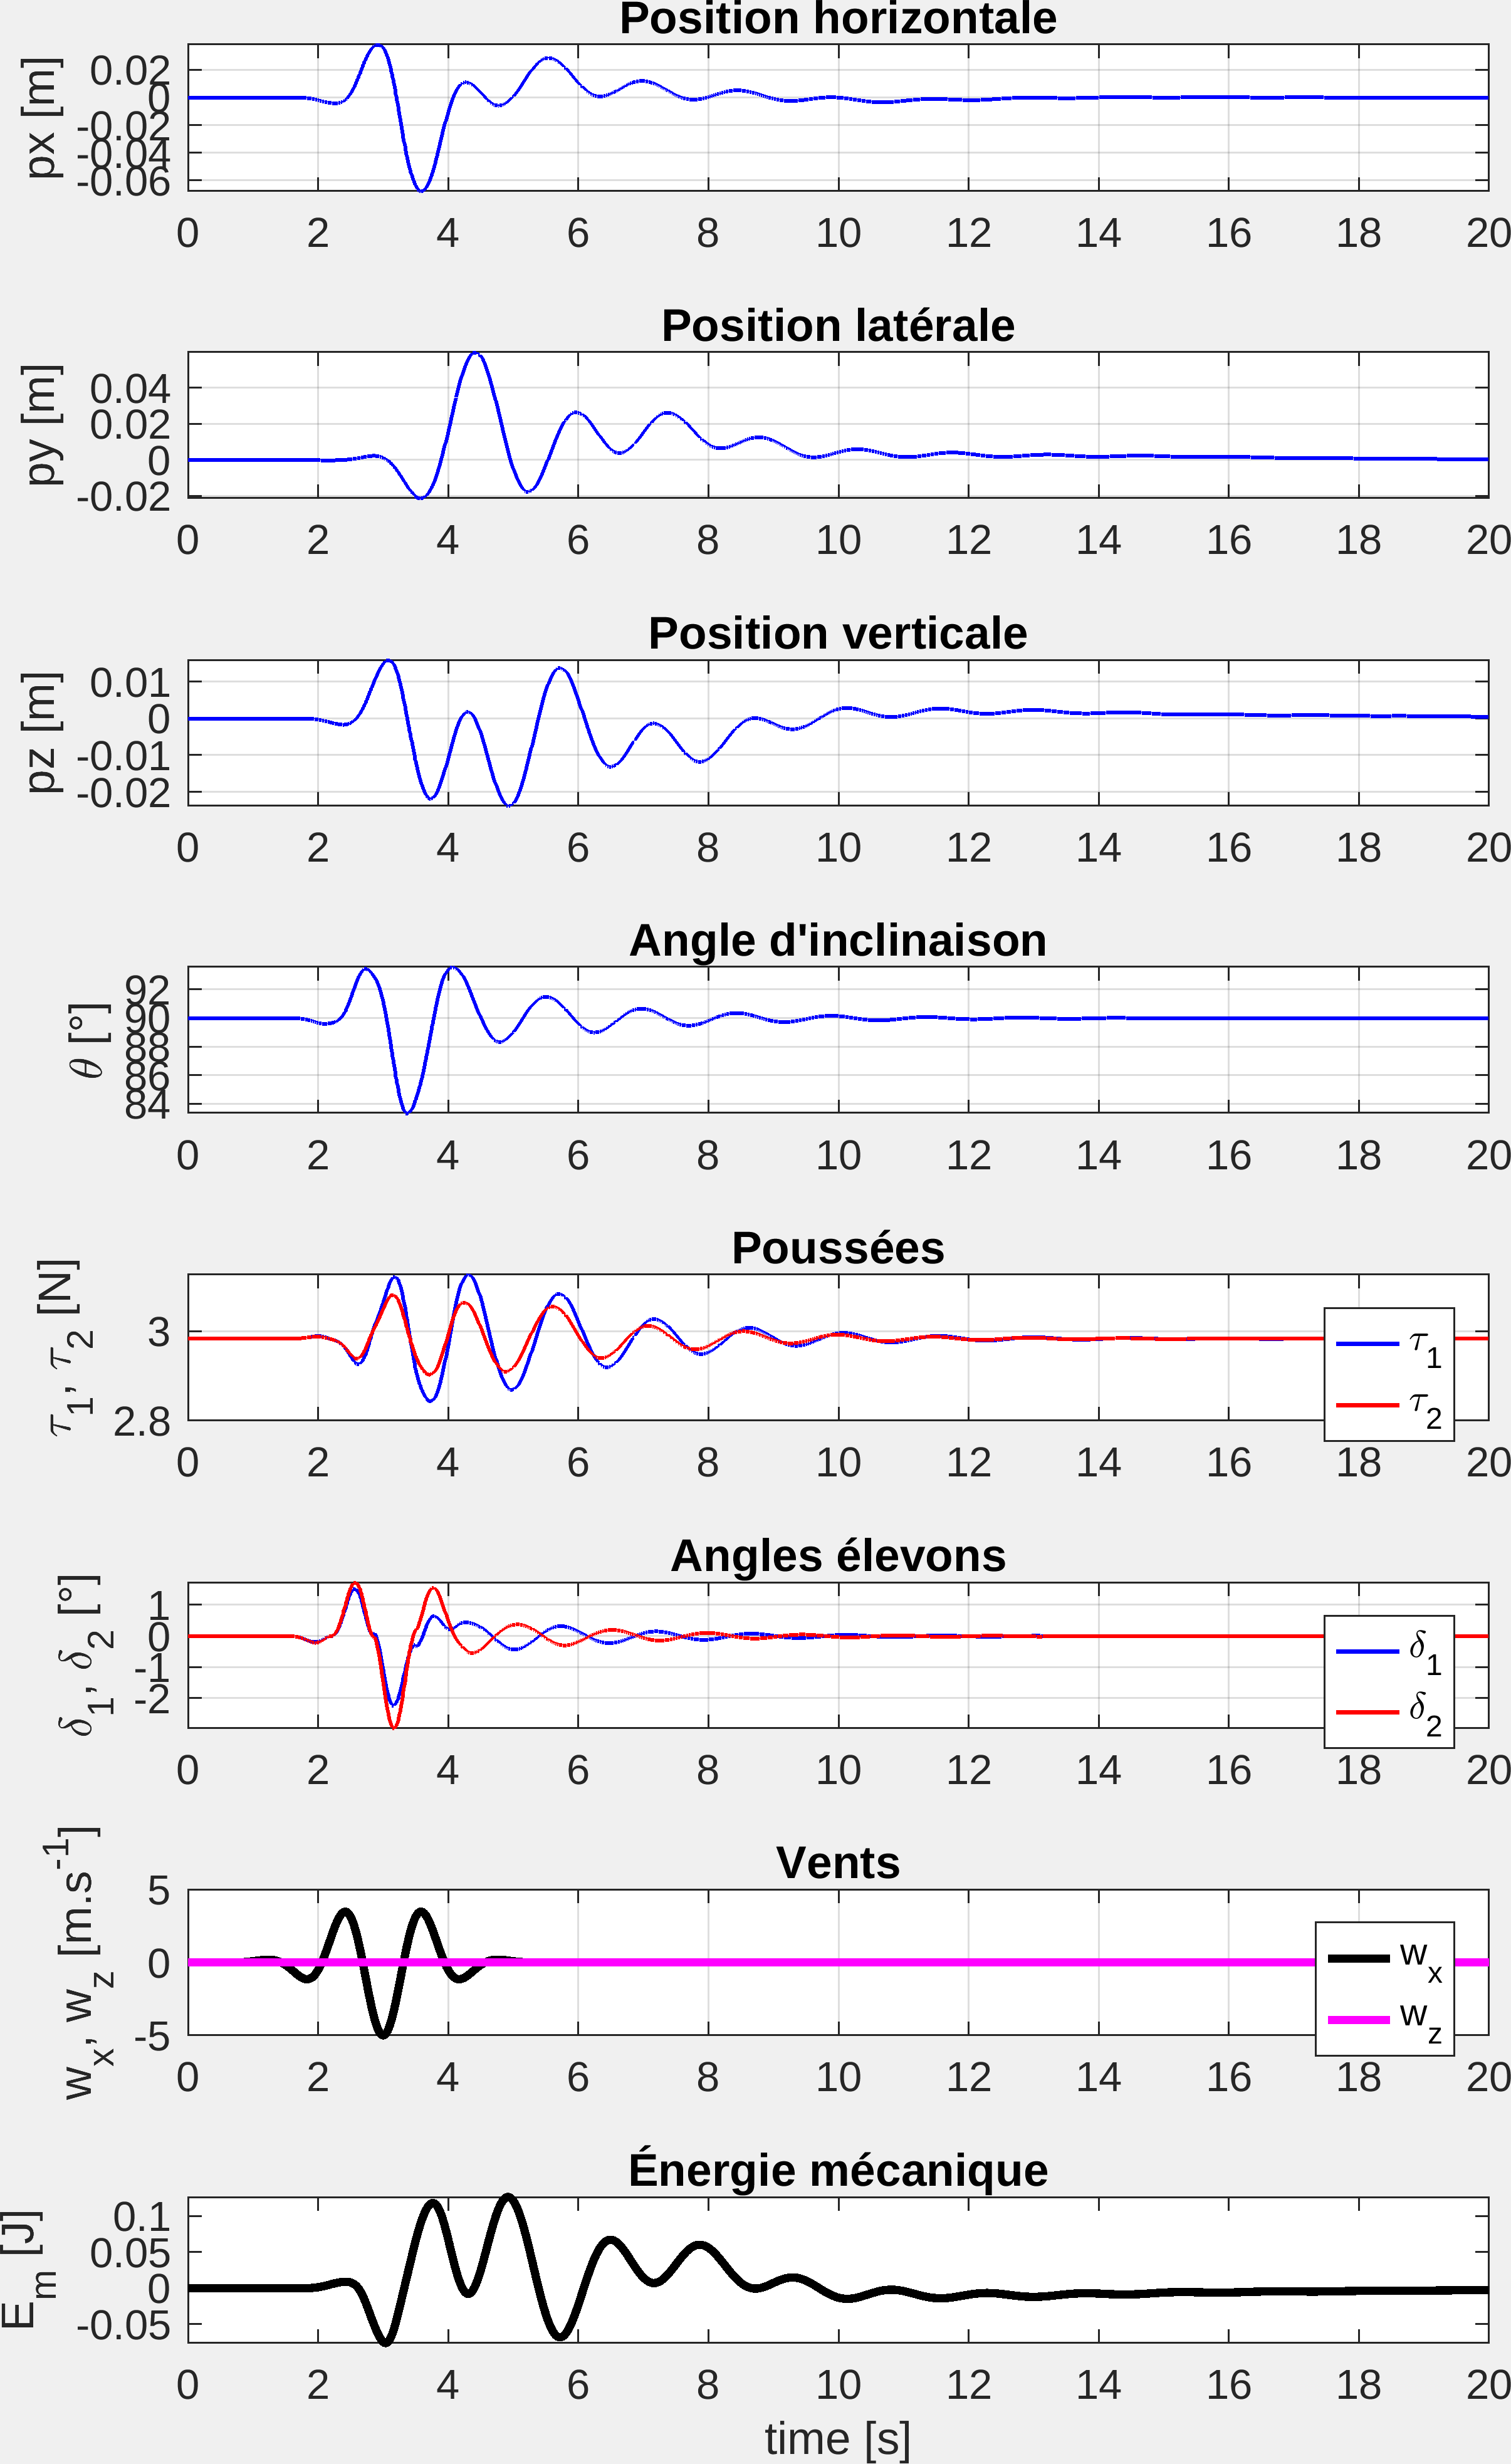
\includegraphics[width=0.33\textwidth]{figures/sim_mor5ms.png}
    \quad
    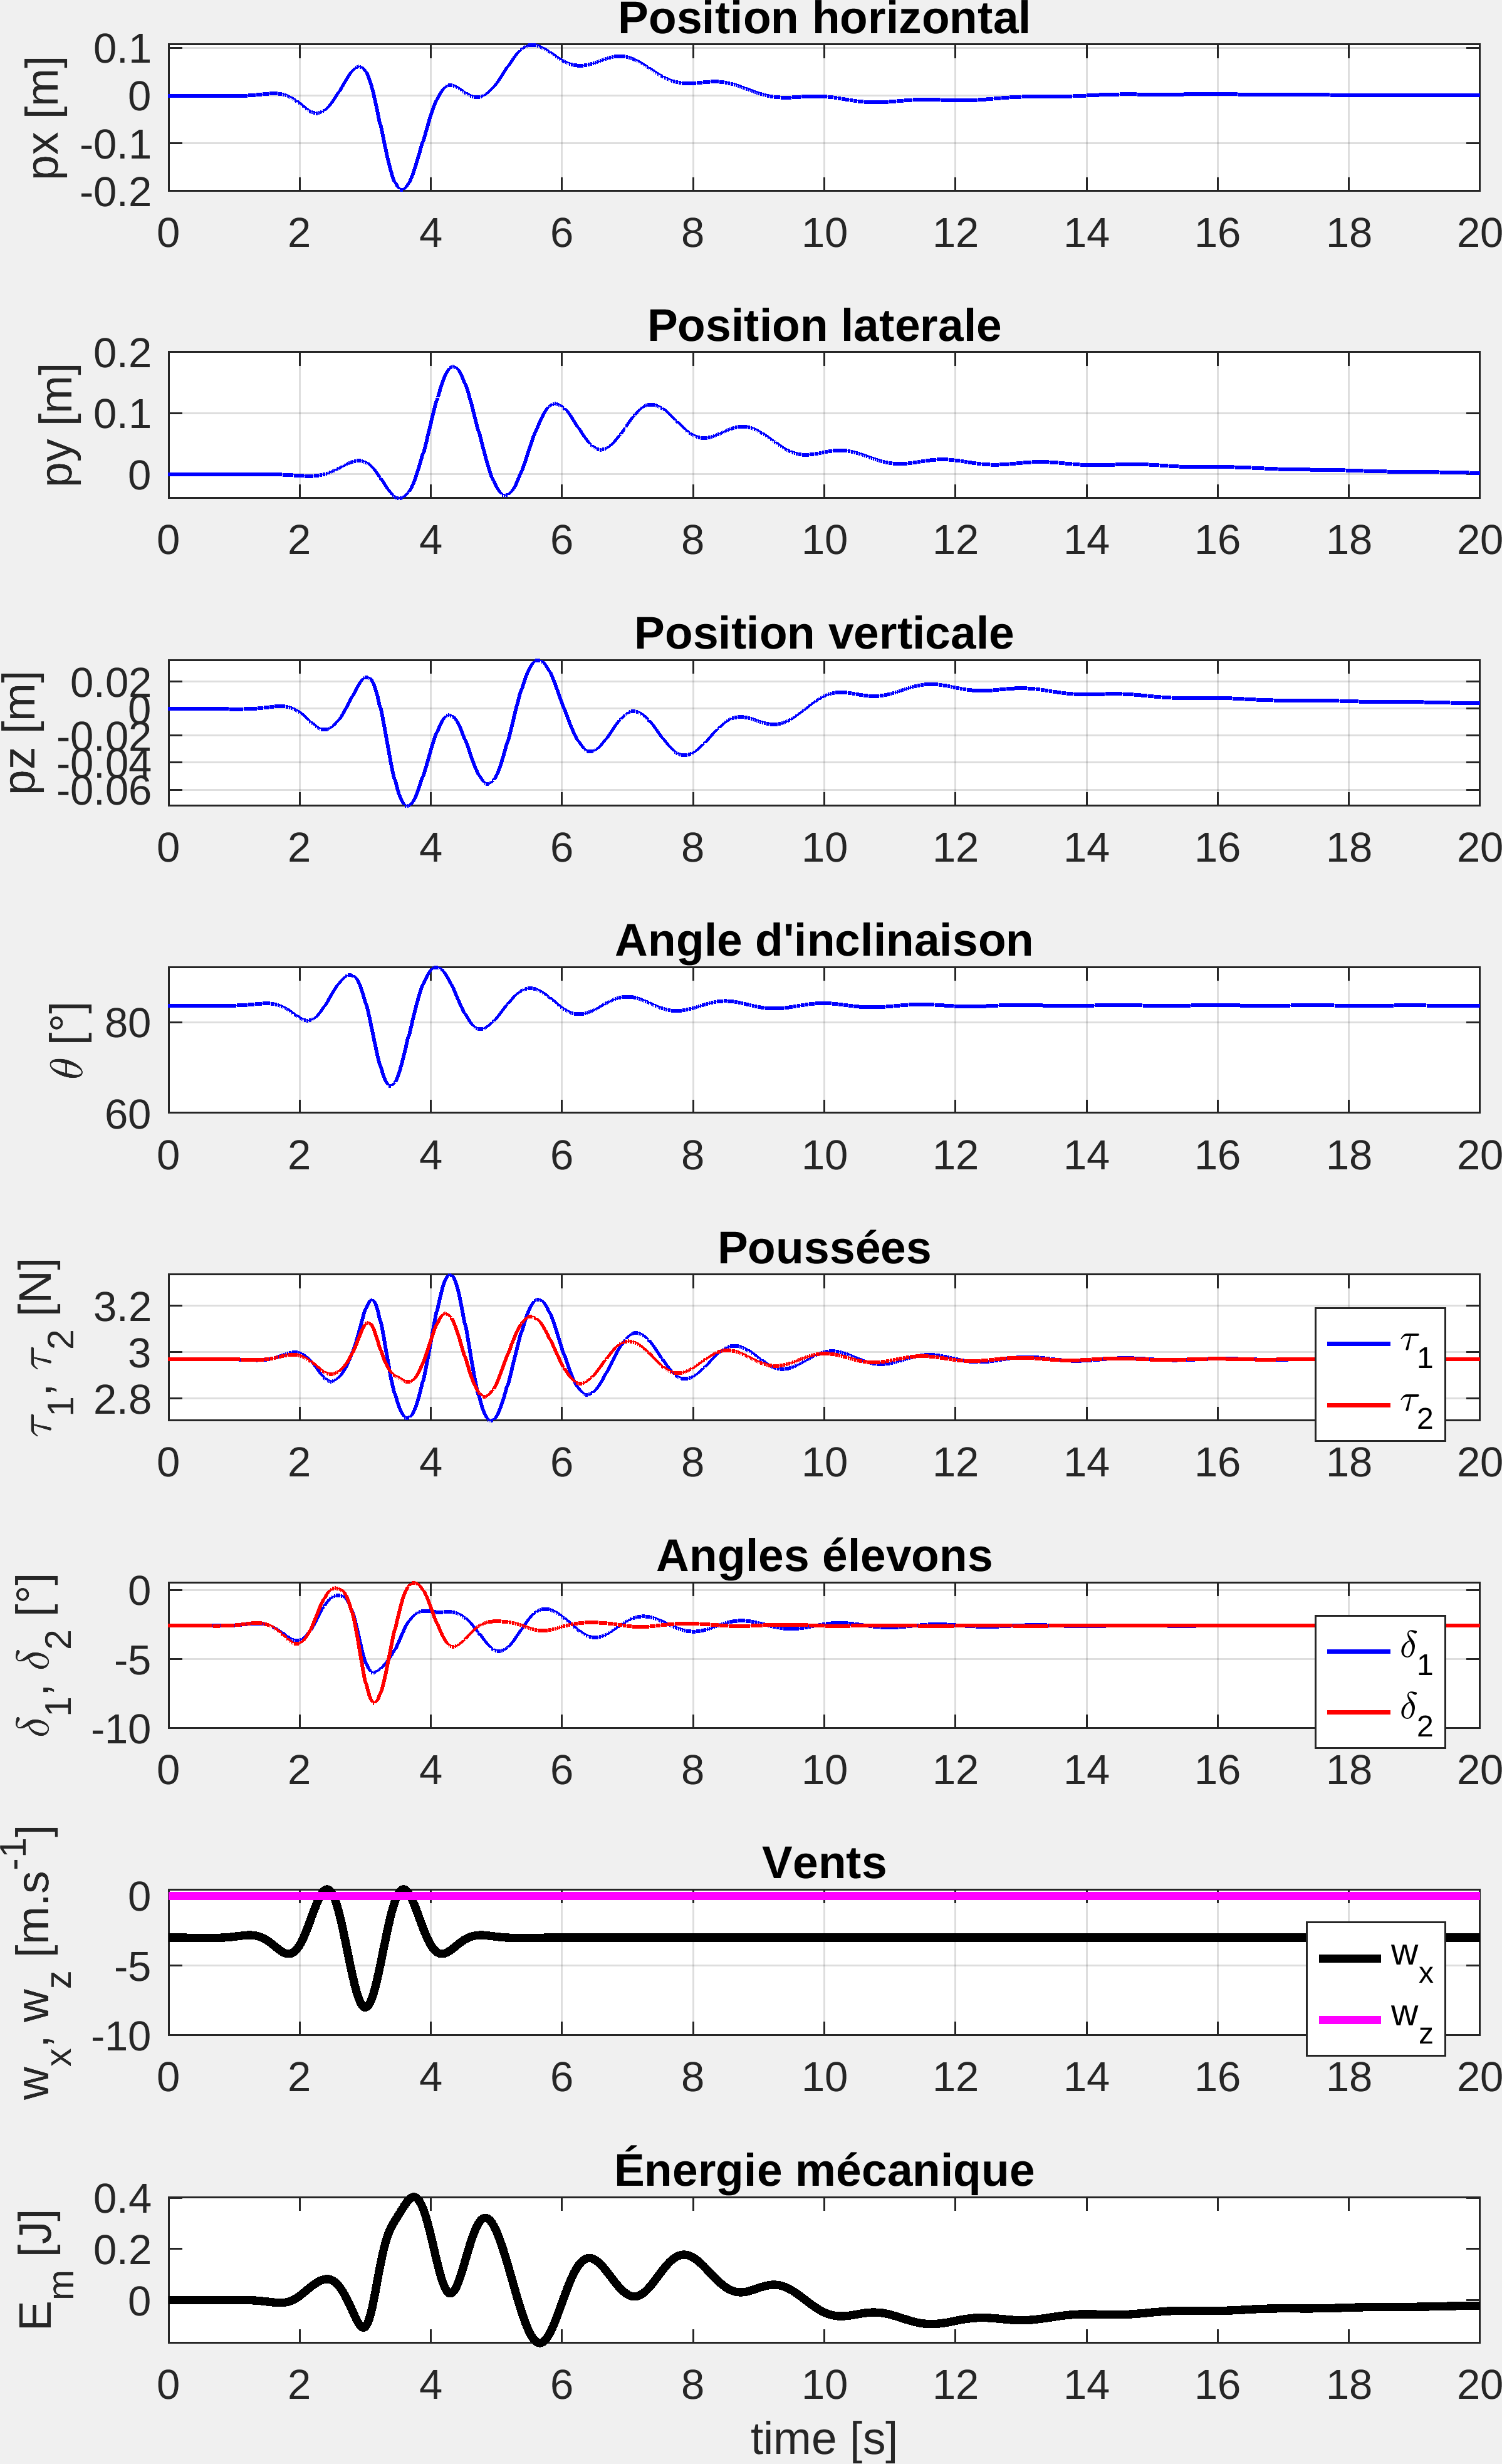
\includegraphics[width=0.33\textwidth]{figures/sim_mor8ms.png}
    \quad
    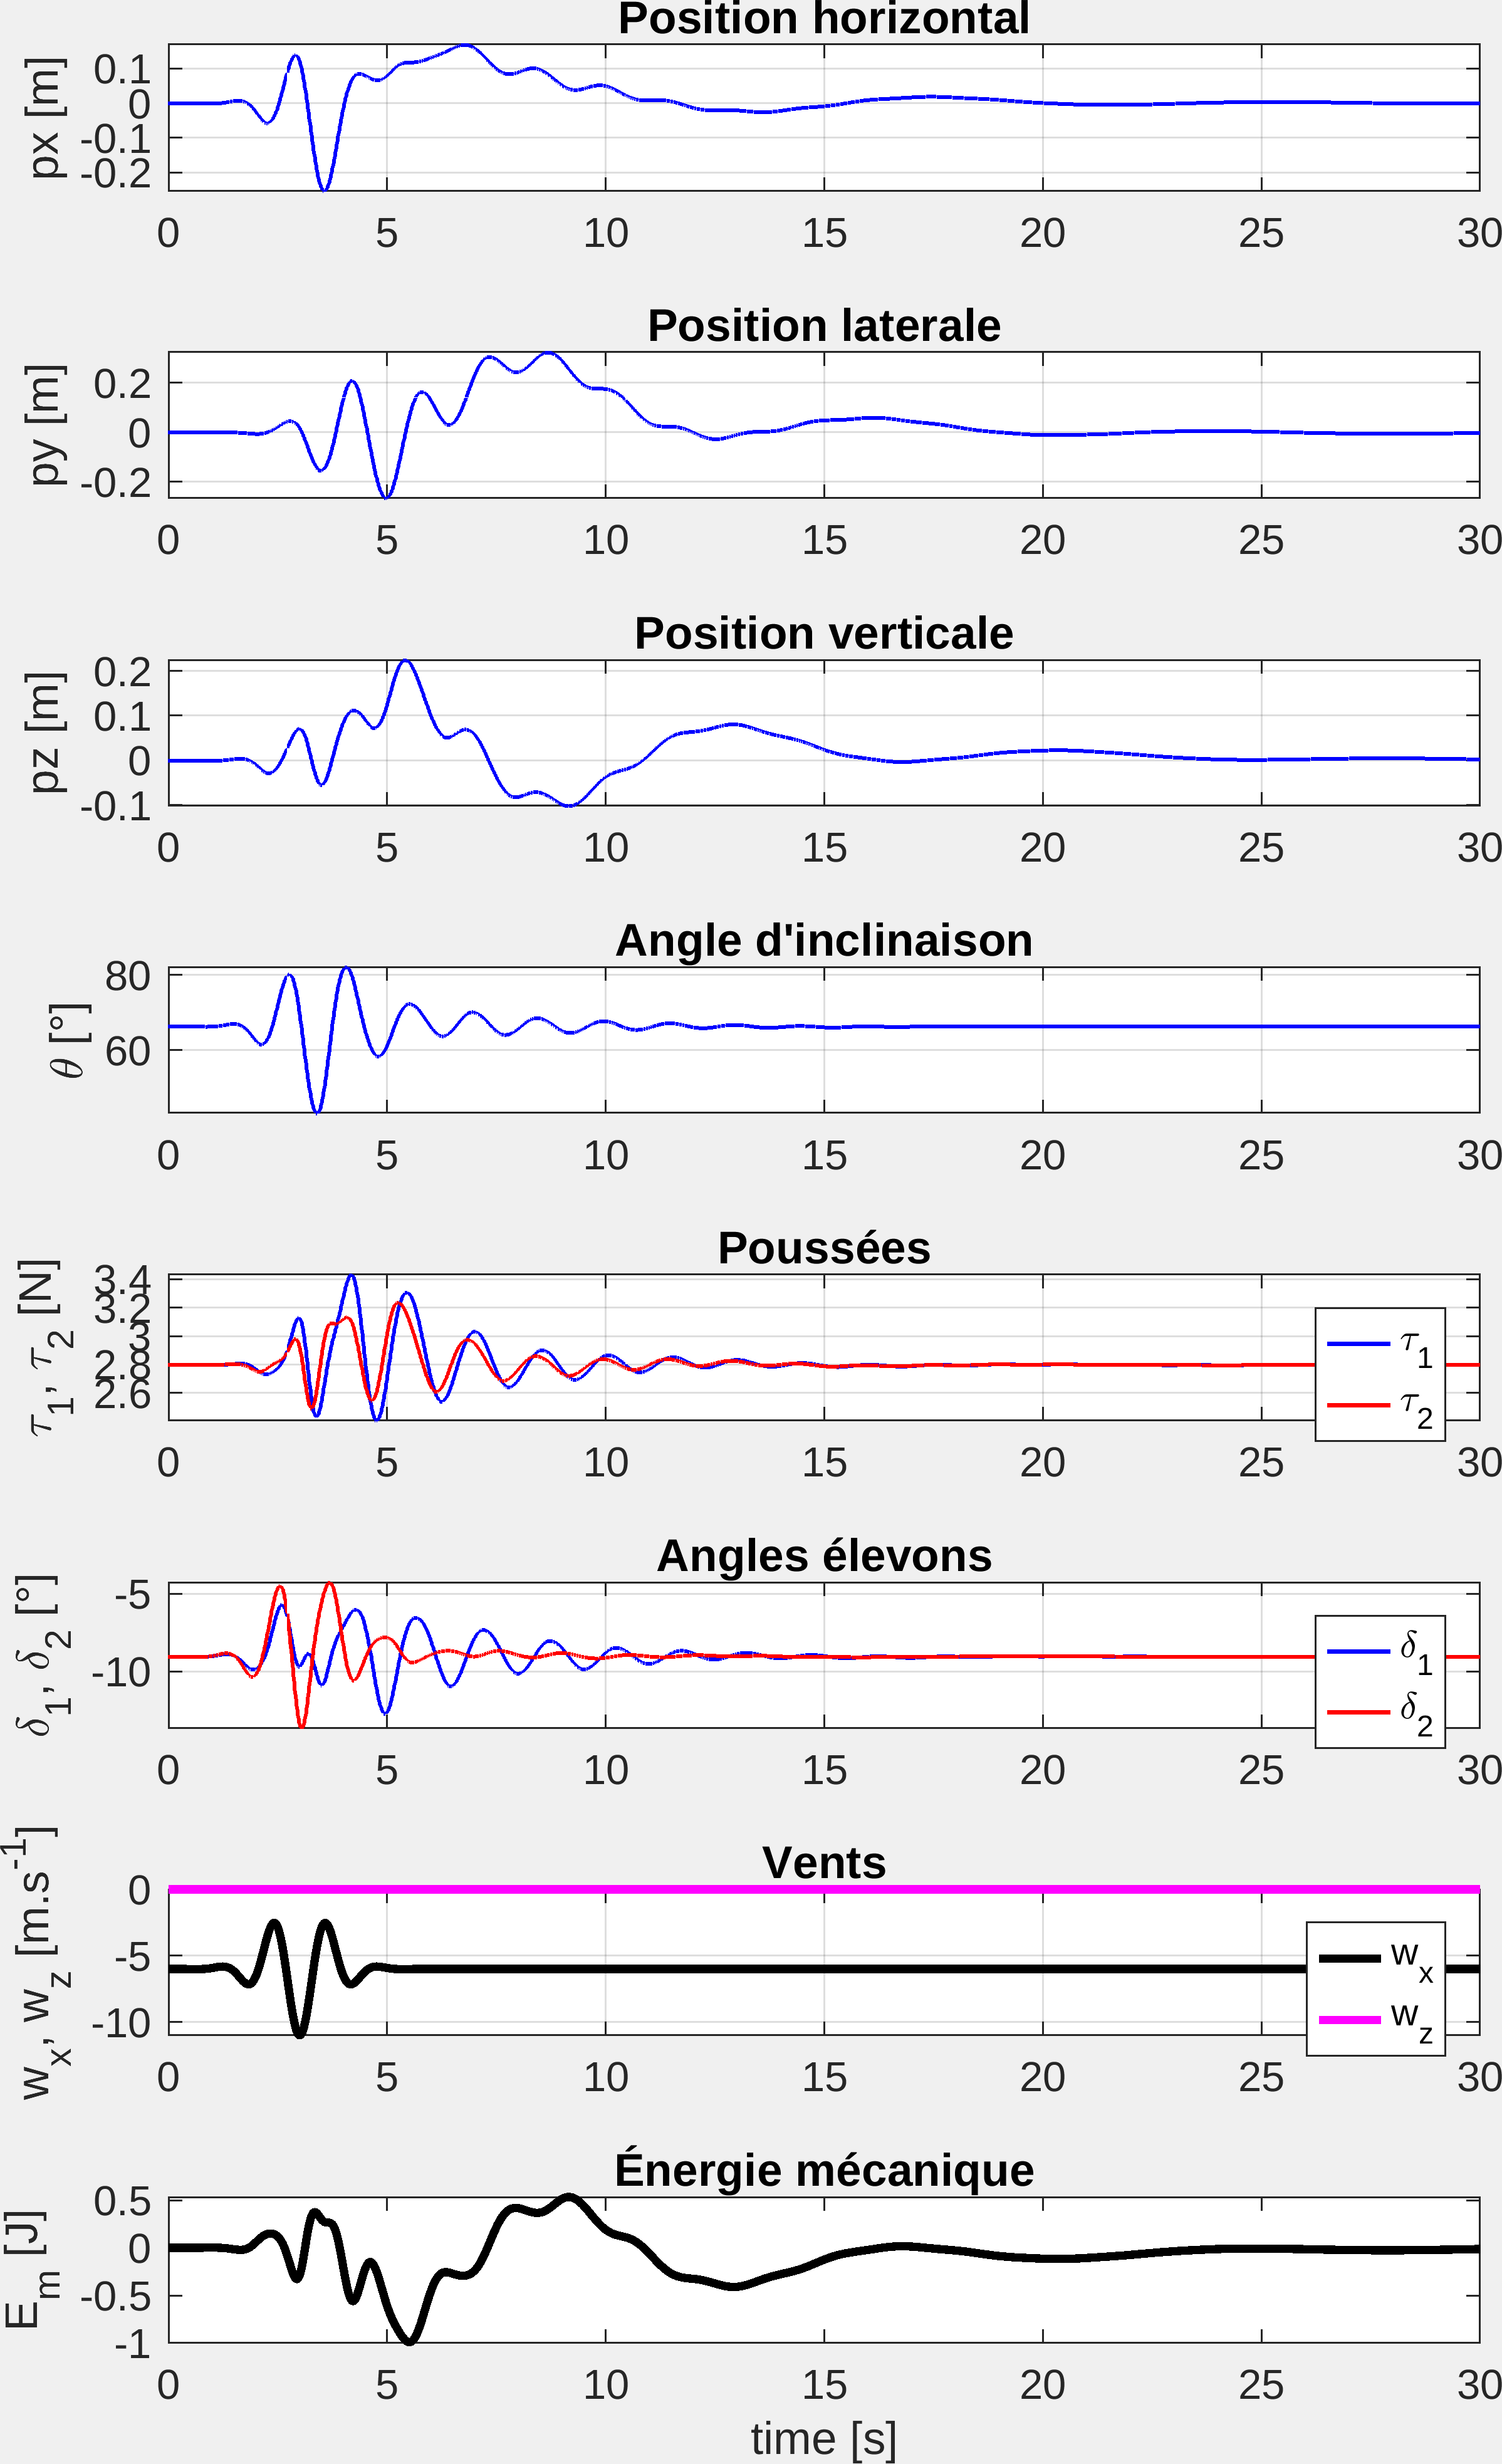
\includegraphics[width=0.33\textwidth]{figures/sim_mor11ms.png}
    }
    \caption{Simulation du modèle non linéaire \eqref{eq:dyna_orig} face à une perturbation "ondelettes de Morlet" \eqref{eq:morlet}.}
    \label{fig:sim_morlet}
\end{figure}
Nous observons que le drone et son contrôleur sont en mesure de rejeter les différentes perturbations.
Nous observons sur l'ensemble des simulations que le drone lutte contre le vent incident en modifiant son incidence, il s'aligne dans le flux du vent, ce qui à pour impact majeur de faire prendre de l'altitude au drone.


\section{Vol expérimental en soufflerie ouverte} 
\label{sec:exp6DOF}

Les vols expérimentaux de DarkO se sont déroulés dans un espace dédié (voir Fig.~\ref{fig:flight_windshape}) avec un système de localisation Optitrack basé sur une convention NED selon la Figure~\ref{fig:darko2}. Nous avons utilisé un générateur de vent à veine ouverte pour obtenir des incréments de vent que nous avons mesurés à l'aide d'une sonde à fil chaud (la barre verticale dans la Fig.~\ref{fig:flight_windshape}). 
\begin{figure}[ht!]
    \centering
    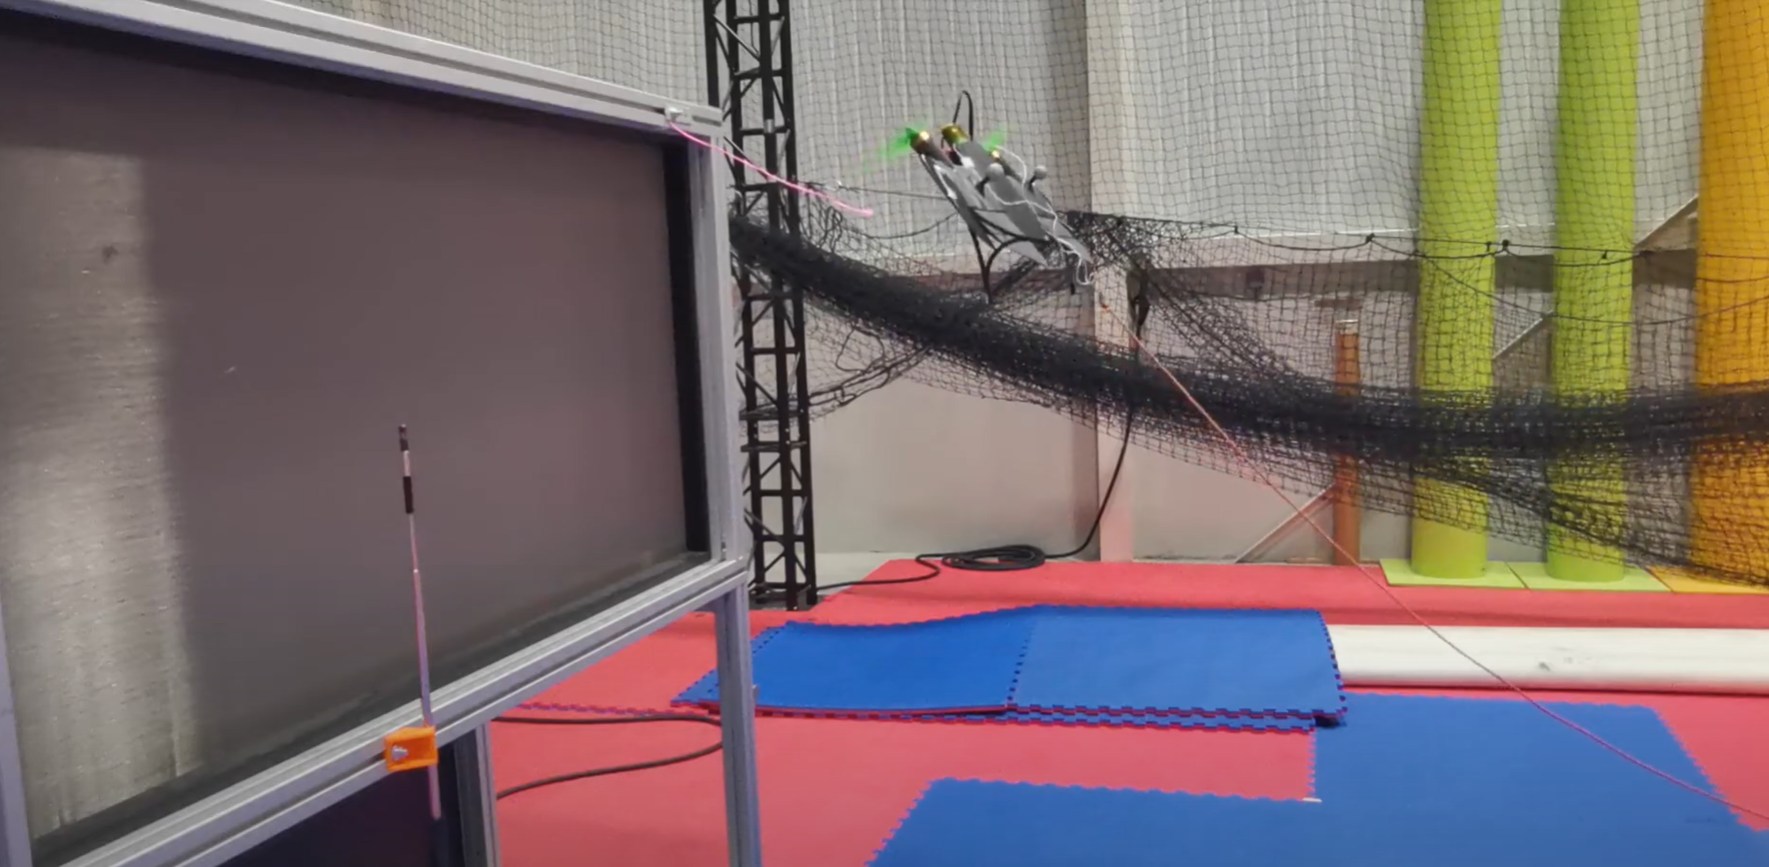
\includegraphics[trim=0cm 0cm 0cm 0cm,clip,width=0.6\columnwidth]{figures/img_flight_darko.png}
    \caption{Vol expérimental de DarkO devant la soufflerie ouverte.}
    \label{fig:flight_windshape}
\end{figure}
Bien que cette information sur le vent soit enregistrée à bord du drone pour synchroniser les données, nous n'utilisons pas cette mesure dans la loi de commande. La fréquence de mesure de cette sonde de vent n'est que de 0,5 Hz, de sorte que nous n'avons qu'une mesure toutes les deux secondes. 
L'estimation de l'état est effectuée à l'aide d'un système de navigation inertielle pour fusionner les données de l'unité de mesure inertielle (IMU) et du système de localisation Optitrack afin d'obtenir une estimation précise de la sortie $\boldsymbol{y}$ dans la Fig.~\ref{fig:commande_int6DOF}. Cependant, la vitesse angulaire du drone $\boldsymbol{\omega}_{text{b}}$ est mesurée sur la base du gyromètre de l'IMU, qui fournit des mesures bruitées. Nous avons donc ajouté un filtre passe-bas \textit{Butterworth} de second ordre avec une fréquence de coupure de 20 Hz pour lisser la sortie $\boldsymbol{\omega}_{text{b}}$. Le filtre de \textit{Butterworth} est pris en compte dans la dynamique linéarisée lors de l'optimisation des gains du contrôleur en suivant l'Algorithme~\ref{alg:iterativeOptimisation}. 

\begin{figure}[ht!]
    \centering
    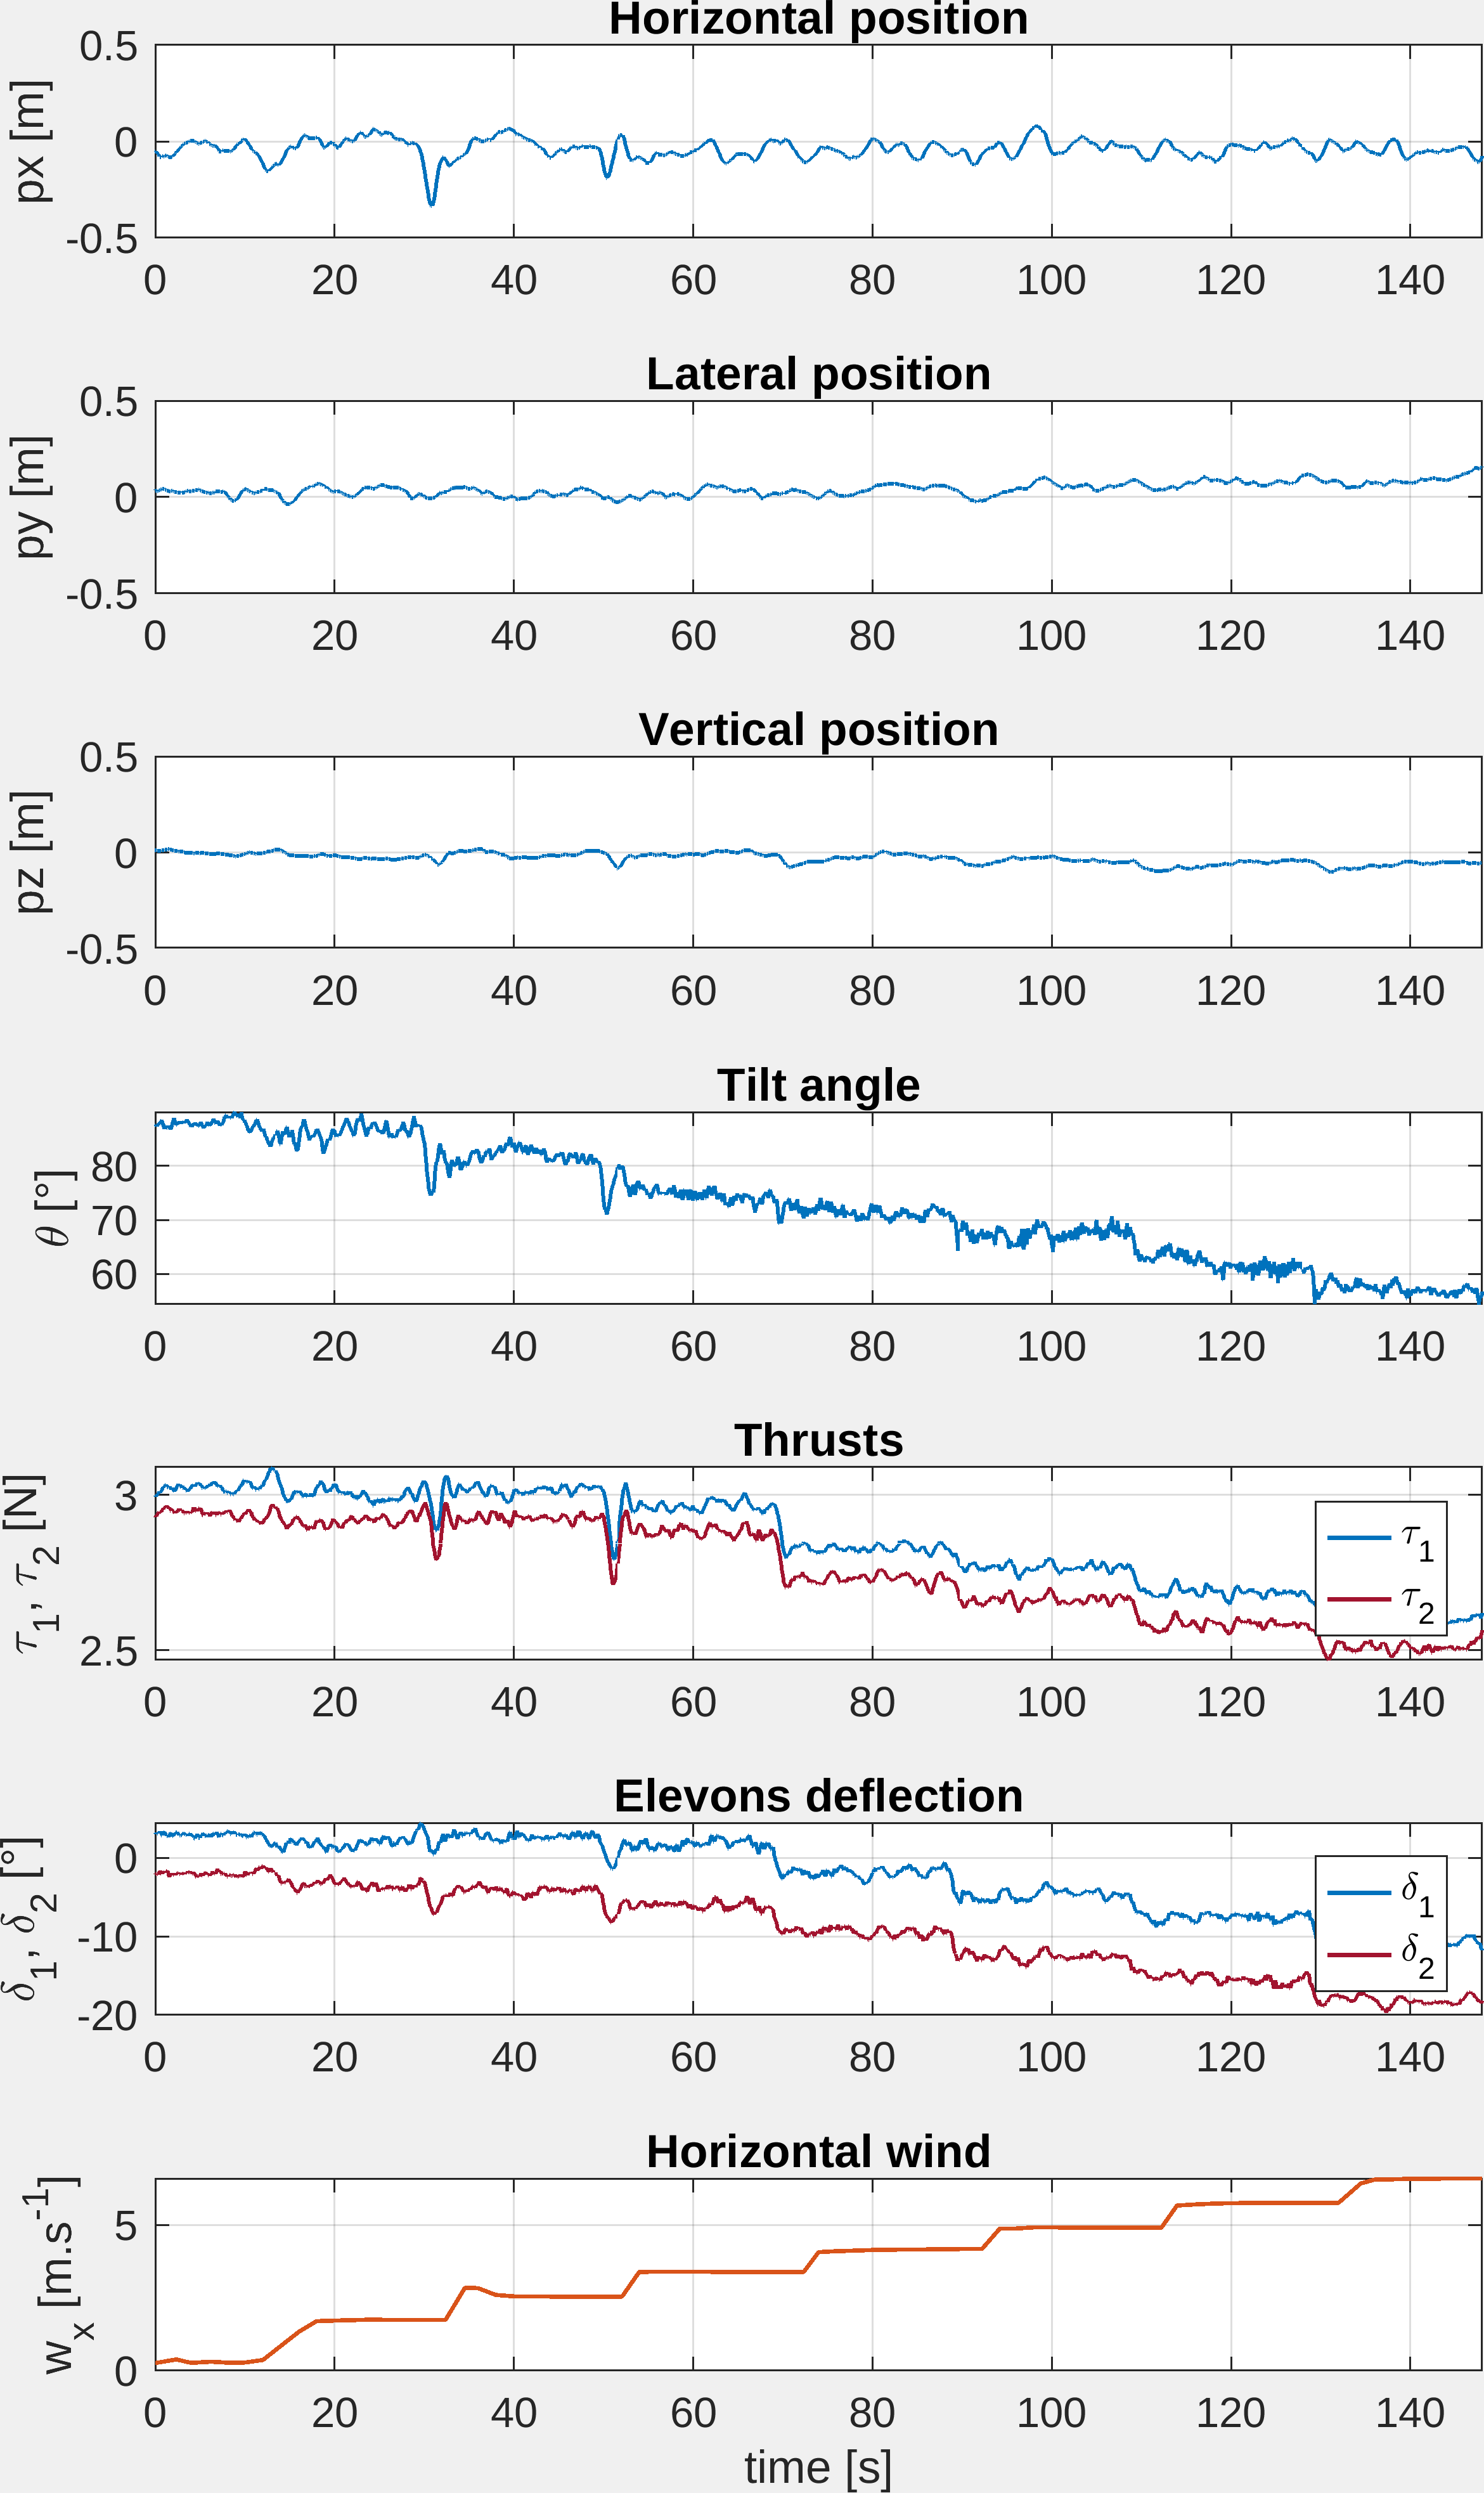
\includegraphics[trim=0cm 0cm 0cm 0cm,clip,width=0.6\columnwidth]{figures/exp_systune_struct.png}
    %'/home/florian/Log/DarkoLog/09_11_23/23_11_05__06_40_06_SD.data'
    \caption{Expérience du drone DarkO devant la soufflerie avec des incréments de vent constants croissants (graphique du bas).}
    \label{fig:ExpSytuneStruct}
\end{figure}

Nous avons également utilisé les ESC similaires à ceux utilisés lors de l'identification montrée dans la Figure~\ref{fig:IOmot} pour l'actionnement des hélices. Les deux ESC ont été flashés avec le code open-source AM32 (voir Annexe \ref{sec:AM32}). De cette manière, nous compensons les effets de décharge de la batterie et obtenons un suivi précis de la vitesse commandée. Avant cette modification, l'action intégrale de la rétroaction stabilisatrice de la Fig.~\ref{fig:commande_int6DOF} compensait la perte de vitesse du moteur causée par la réduction de la tension de la batterie pendant le vol. Cette compensation intégrale a été indirectement générée par la perte d'altitude du drone causée par la réduction de la traction. 

Nous avons réalisé une expérience de vol au cours de laquelle DarkO a été mis manuellement en mode de vol stationnaire stabilisé devant la soufflerie, puis nous avons activé la loi de contrôle de l'Algorithme~\ref{alg:iterativeOptimisation}. Comme le drone devait être stabilisé à au moins \SI{30}{\centi\meter} de la soufflerie, un pilotage manuel a été réalisé pour éviter tout dépassement qui pourrait endommager la soufflerie. Une fois que DarkO était suffisamment proche du point de consigne $\boldsymbol{r}_{p}$ de la Fig.~\ref{fig:commande_int6DOF}, nous avons activé le contrôleur proposé, obtenant les résultats de la Fig.~\ref{fig:ExpSytuneStruct}. Au cours de la phase d'expérimentation, comme le montre le graphique inférieur de la Fig.~\ref{fig:ExpSytuneStruct}, nous avons augmenté progressivement la vitesse du vent, en attendant 20 secondes entre chaque évolution de vent jusqu'à une vitesse finale de \SI{7}{\meter\per\second}.


\begin{figure}[ht!]
    \centering
    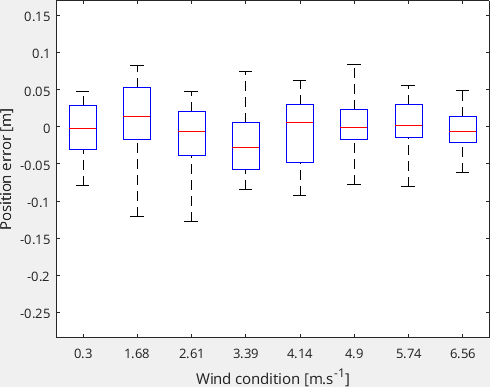
\includegraphics[trim=0cm 0cm 0cm 0cm,clip,width=0.6\columnwidth]{figures/boxplot.png}
    \caption{Visualisation statistique des performances de vol stationnaire.}
    \label{fig:statpos}
\end{figure}

Les figures~\ref{fig:ExpSytuneStruct} et~\ref{fig:statpos} montrent que le drone maintient sa position malgré l'augmentation de la vitesse du vent. Nous pouvons noter quelques points importants, en accord avec les simulations : la traction du moteur diminue lorsque la vitesse du vent augmente. Le schéma de contrôle profite de la portance générée par le vent pour soutenir le drone, de sorte que moins d'énergie soit nécessaire pour stabiliser la position en vol stationnaire. Le drone maintient son angle d'inclinaison à une valeur inconnue, a priori, pour la loi de commande et qui découle naturellement de l'action intégrale. Cette valeur est atteinte asymptotiquement et converge vers la valeur requise de $\theta$. Pour stabiliser la position, le drone utilise les élevons pour annuler le moment de tangage généré par la forme de l'aile, soumise à un vent horizontal, sans atteindre les limites de saturation.
On note également une légère asymétrie de l'efficacité des actionneurs, qui est efficacement compensée par l'action proportionnelle du schéma de contrôle.


\section{Conclusion du Chapitre \ref{chap:6DOF}}
Nous avons proposé un schéma de contrôle pour la stabilisation d'un \textit{tailsitter} lors d'un vol stationnaire en présence d'un vent constant inconnu. Notre bouclage contient une action intégrale et ne nécessite pas la mesure de la vitesse du vent. Les modèles paramétriques linéarisés se sont avérés être un instrument clé pour effectuer le réglage des paramètres du contrôleur.
Après avoir étudié les résultats de la simulation, nous avons mené une campagne de vols expérimentaux dans un environnement contrôlé pour valider notre solution de contrôle. 

La principale limitation de cette architecture réside dans l'impossibilité de mesurer le vent dans les phases de vol stationnaire ou de vitesse faible. Pour tenter de résoudre ce problème, nous avons proposé une nouvelle architecture.


